
\begin{savequote}
Computers are useless. They can only give you answers.
\qauthor{Pablo Picasso}
\end{savequote}

\chapter[Automatic Classification of NVC]{Automatic Classification of NVC in Spontaneous Conversation}
\label{ChapterClassification}
\label{SectionClassificationIntro}

\thesiscomment{MAIN POINT OF CHAPTER: Generalising heuristic geometric features into an algorithmic set is an effective approach for binary classification of clear, person independent examples of \ac{NVC} signals for both forward and backchannel signals.}

This chapter describes a study of automatic recognition of natural \ac{NVC} in informal conversations. To find the features and classifier best suited for this task, a comparison between various alternative components of the recognition system is performed. The automatic system uses the naturalistic \ac{NVC} corpus described in the previous chapter.
%\ac{NVC} includes all types of communication except the literal spoken words. \ac{NVC} uses multiple modalities including visual, audible, spatial and tactile signals. 
This thesis only considers visual information, because it is an important mode for \ac{NVC}. Although the exact modality distribution of each \ac{NVC} is not well documented in the literature, possibly due to the enormity of such a task, this study focuses on facial behaviour because it is obviously a very significant modality for \ac{NVC}\footnote{``In fact, some researchers believe the primary function of the face is to communicate, not to express emotions.'' \cite{Knapp2009}, p. 9}. However, other non-facial behaviours are thought to play a significant role in the expression of \ac{NVC}. Also, it is well known that the non-verbal component of voice contains sufficient information to recognise emotion. %by humans and automatically
It is likely that a hybrid approach using visual and audio information would be an effective approach for \ac{NVC} recognition.

%Almost all previous studies of automatic behaviour recognition occur in controlled or artificial situations. For some applications this is acceptable, but for \ac{NVC}, which is largely influenced by social context, acted human behaviour is unlikely to be useful in training a practical system. The naturalistic corpus described in the previous chapter is used. 
Because the TwoTalk corpus is used for training, this is one of the first automatic \ac{NVC} recognition systems to operate on informal conversation \footnote{The existing AMI corpus contains informal conversation and has been used for automatic recognition but the labels used generally do not address \ac{NVC} specifically.}. It is also one of the first to recognise human behaviour outside of a task based, role play based or otherwise specialised situation \footnote{Again, some studies have used the informal part of the AMI corpus has been addressed, but often these studies also consider the acted data as they are part of the same data set.}. 
%Arguably one major deficiency with our corpus is it is still recorded in a studio laboratory. Corpuses for automatic systems of naturalistic behaviour outside the laboratory have only recently become available. 
This chapter only uses clear samples of \ac{NVC}, while intermediate intensity samples are discarded (this is discussed in detail in Section \ref{SectionClearExamples}). This simplifies the recognition task and makes the work similar to some previous studies which use strong acted emotion, while retaining the naturalistic quality of the data. However, a practical system should also operate on intermediate intensity \ac{NVC}; this issue is considered in Chapter \ref{ChapterNvcRegression}.
There are only a few previous studies of automatic \ac{NVC} recognition, with agreement and disagreement being the most popular. 
%Of course, there are many other papers on emotion, facial expression, social dynamics, and internal state of people. In contrast, this thesis attempts to use labels that correspond to the meaning of intentional communication acts. As previously discussed, this haves many potential applications in \acf{HCI}. 
The annotation labels used in this thesis are \textit{agree}, \textit{thinking}, \textit{question} and \textit{understand}. 
%These \ac{NVC} signals frequently occur in many social situations and across cultures. The annotation was performed by multiple annotators and their ratings were averaged to form a consensus.

The primary contributions of this chapter are:

\begin{itemize}
\item A study of automatic \ac{NVC} classification of clear, naturalistic samples in informal conversation. Different approaches to \featureGeneration and classification are compared.
\item Visualisation and analysis of \textit{thinking} \ac{NVC} in a simplified feature space based on eye movements, to determine the presence of any consistent behavioural patterns.
 %several feature extraction methods for \ac{NVC} classification, with two classifiers. %Geometric shape features with an \ac{SVM} classifier exceeded the performance of the other methods that were tested. A features set based on distances between pairs of trackers was found to be effective, and has better generalisation to unseen people.
\item An analysis of classification performance for specific types of \ac{NVC} signals, to find their relative recognition difficulties.%Evidence that some \ac{NVC} categories are comparatively easy to recognise and others are relatively difficult: \textit{question} and \textit{understand} are harder compared to \textit{agree} and \textit{thinking}.
\item A comparison between the feature extraction approach and temporally encoding the features using a quadratic function. %This approach does not result a significant performance increase for \ac{NVC} recognition.
\end{itemize}

%Chapter \ref{ChapterLiteratureReview} discussed \ac{NVC}, classification methods and \featureGeneration. The corpus was described in the previous chapter. 
The following section provides an overview of existing classification techniques. Section \ref{SectionClassificationOverview} provides a broad overview of the automatic system. Section \ref{SectionFeatureGeneration} explains the various \featureGeneration methods used in the comparison. Various \featureGeneration methods are compared to determine the best approach. Section \ref{SectionClassificationMethods} describes the classifiers used in the comparison. The selection of clips for training and testing from the corpus is described in Section \ref{SectionClearExamples}. Performance measurement is detailed in Section \ref{SectionClassificationPerformance}. The performance of various features and classifiers is shown and discussed in Section \ref{SectionNvcClassificationResults}. The use of polynomial curves to encode temporal variations is examined in Section \ref{SectionTemporalFeatures}. An exploration of \textit{thinking} in a simplified feature space is conducted in Section \ref{SectionVisualisingGaze}. Work by Akak{\i}n and Sankur \cite{Akakin2011} that builds upon the work of this chapter is discussed in Section \ref{SectionHmm}.

\section{Overview}
\label{SectionClassificationOverview}

\begin{figure}[tb]
\centering
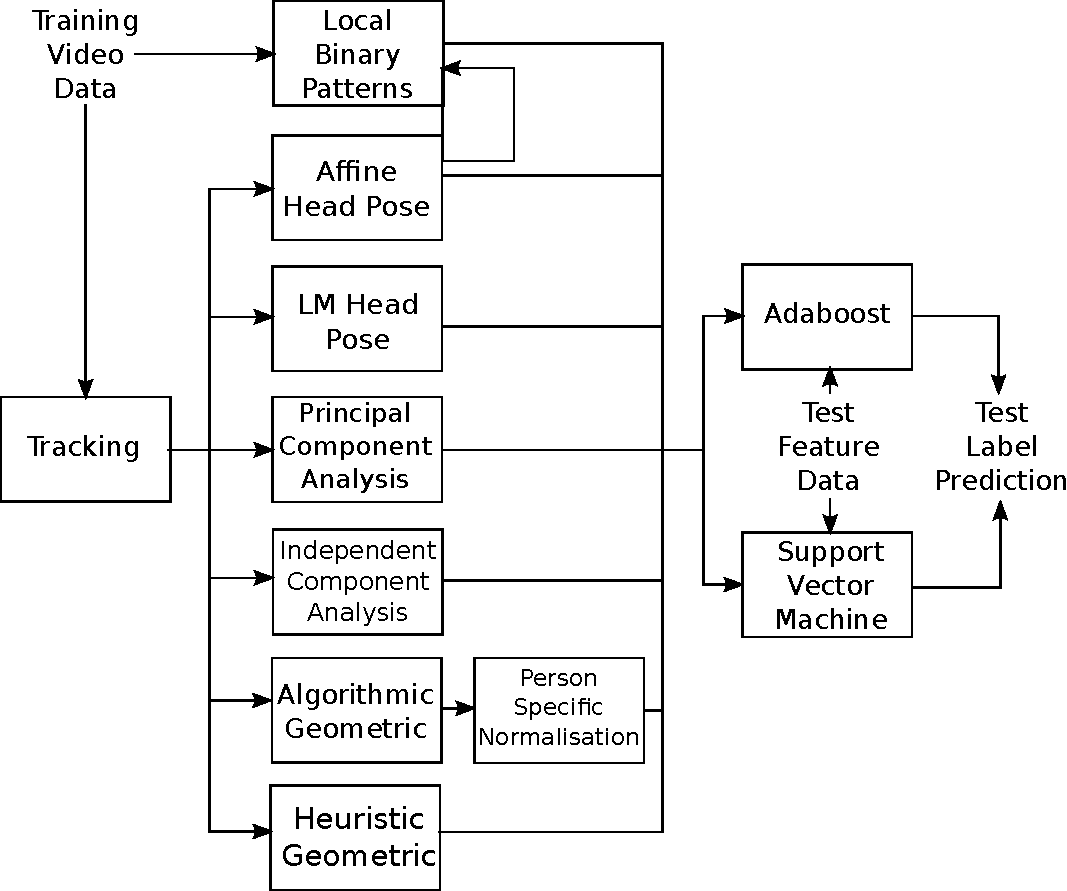
\includegraphics[width = 0.6 \columnwidth]{nvcclass/classSystemOverview.pdf}
\caption{An overview of the automatic \ac{NVC} classification system.}
\label{FigureClassificationOverview}
\end{figure}

This chapter describes an automatic \ac{NVC} classification system and evaluates its performance. 
%This section provides a brief overview of what stages are involved and how they are related. 
The basic steps are shown in Figure \ref{FigureClassificationOverview}. Corpus data is split into cross validation folds of seen training data and unseen test data. 
%Tracking and various \featureGeneration methods are applied to the digital video frames to reduce the effect of irrelevant changes. 
Various \featureGeneration techniques are used as the baseline for a comparison of different approaches. The features are then used to train either an \ac{SVM} or Adaboost model. The model is used to predict labels on test data, on which the appropriate \featureGeneration technique has been applied. The predicted labels are compared to annotator ratings and the performance is evaluated.

%Only clear examples of positive and negative \ac{NVC} are used because this simplifies the problem and expressing the problem as a classification task enables many popular machine learning tools to be applied. 
%This pre-processing of clear examples and annotation data is discussed in the following section.

The next section describes the issues in converting the original videos into suitable features for supervised learning.

\section{\FeatureGenerationTitle}
\label{SectionFeatureGeneration}

This chapter describes several different \featureGeneration approaches and compares their performance for \ac{NVC} classification.
%Automatic recognition systems are used to make a prediction on unseen samples based on input data. This input data is often from sensor equipment, such as a photo or video camera. In many applications, using the raw data directly from the imaging device usually leads to poor results. This is due to poor class separability in the raw data input space. Feature generation is the process that maps raw input data into a higher level feature space that has better class separation. 
\FeatureGeneration takes raw input frames and produces a feature representation that is intended to increase the robustness to changes in the raw input data that are not significant for the application.
%Because of the need to isolate meaningful changes from those that are irrelevant, the type of feature selection used is largely application specific. Determining which features are optimal is also not obvious, because the possibilities for \featureGeneration approaches are unlimited. Given that there are an infinite number of non-linear transforms that map the raw input space to a space with perfect class separation, a particular approach cannot be assumed to generalise to unseen test data. Because there are no cross domain automatic \featureGeneration strategies, the \featureGeneration method used is typically selected by a human expert. Another potential advantage of \featureGeneration is that generated feature vectors are often more compact than the original input data. I will now discuss how \featureGeneration applies to \ac{NVC} recognition.
%Previous studies found that there is a great deal of information conveyed by the human face and head (see Section \ref{BackgroundHowIsNvcExpressed}). Other types of \ac{NVC} signals are thought to exist apart from the face but they are not considered in this study. The most obvious non-visual mode that conveys \ac{NVC} is audible non-verbal information, particularly the non-verbal component of a voice. Gesture might also be worth studying, as it probably has a role in conveying \ac{NVC} signals of interest. Some of these communication modes were not recorded as part of the corpus (e.g. hand position). However, given the complexity of encoding this information and the many possible approaches of combining features of different forms, multi-modal communication was judged to be too broad an issue to address in this thesis.
%The raw input data is in the form of digital video frames. Relevant information needs to be encoded that reflects the face shape and appearance, while ignoring irrelevant changes in the raw input. 
The irrelevant changes include:

\begin{itemize}
\item identity and face shape,
\item lighting changes,
\item head rotation and translation, although it is useful to have this encoded separately from emotion and not entirely discarded and
\item occlusions.
\end{itemize}

%Although changes caused by relevant face and head motions can be seen in the digital video frames, the relationship is highly non-linear. This is partly caused by the head moving and each pixel does not view a consistent part of the face. To extract the position and motion of the face, feature point tracking is used. Tracking is a form of \featureGeneration, in which the raw input space (video frame data) is transformed into a feature space (tracking positions) in which irrelevant information is partly removed. Although the tracking data encodes information about face shape, the dominant cause of variation in feature space is head translation and rotation. Because natural conversations have a significant component of both, this information should be separated or removed to obtain usable and robust face deformation features. Again, there are many possible \featureGeneration approaches. This chapter presents and compares several methods: \ac{PCA} and \ac{ICA} decomposition, heuristic geometric features and algorithmic geometric features. %What about LBP and head pose?

Existing feature extraction techniques have previously been discussed in Section \ref{BackgroundEncodeFacialInfo}. There are a wide range of possible approaches to facial \featureGeneration and the choice of features in previous works are largely experimentally driven to achieve accuracy on a chosen data set. However, there are a few properties of naturalistic \ac{NVC} that make this task distinct from many posed behaviour based studies. Naturalistic behaviour is harder to recognise than posed examples \cite{Cohn2004b}, probably due to the differences in the way emotions are expressed in these situations, as well as the amount of head pose present in the data. These large pose changes make some approaches unsuitable for natural \ac{NVC} recognition. For this reason, \ac{AAM}s were not used because, in their basic formulation, they are not robust to large head pose changes \cite{Sung2008}. Also, large head pose changes cause significant changes in facial appearance \cite{Lu2006} and normalising face appearance to frontal pose is difficult, requiring image completion or texture synthesis to replace self-occluded parts of the face \cite{Asthana2011}. These factors are likely to make appearance based features less suitable for this task. The effect of large pose changes can be mitigated by the use of a multi-camera recording, but this is a more involved experimental arrangement which limits this approach to fewer practical applications. For these reasons, this study primarily focuses on facial shape recorded using a simple camera. It is assumed that by using the visual modality, only non-verbal communication will be used as the basis for recognition. In principle, it is possible for an automatic system to learn the verbal component of communication via speech reading. However, given the extreme difficulty of speech reading \cite{Ong2011}, this is not a significant factor in the context of this study. The strengths and weaknesses of the methods employed are discussed in the next few sections.

The names of the \featureGeneration approaches have been abbreviated for the sake of convenience: \textit{affine} refers to affine head pose estimation, \textit{deform-cubica} refers to tracking deformations based in CubICA, \textit{deform-fastica} refers to tracking deformations based on FastICA, \textit{deform-pca} refers to tracking deformations based on PCA, \textit{geometric-h} refers to heuristic geometric features, \textit{geometric-a} refers to algorithmic geometric features, \textit{lbp} refers to local binary patterns and \textit{lma} refers to head pose estimation by \acf{LMA} model fitting.

\thesiscomment{TODO Introduce head pose and appearance features.}

%Natural data contains rapid and extreme head motion. The next section describes a pre-existing tracking technique that operates on challenging data.

\subsection{Linear Predictor Feature Tracking for Facial Analysis}
\label{SectionLpTracking}

\begin{figure}
\centering
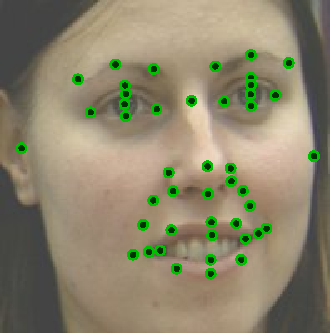
\includegraphics[width = 0.6 \columnwidth]{nvcclass/TrackerPositions.pdf}
\caption{Illustration of position of LP Trackers on facial features.}
\label{FigureTrackerPositions}
\end{figure}

\ac{LP} feature tracking \cite{Ong2009} was applied to unconstrained natural conversation videos. This method was selected because it is relatively robust to head pose changes. The theory for this method is discussed in Appendix \ref{BackgroundLpTracking} and is used instead of the more common trackers, such as \ac{KLT} \cite{Tomasi1991}. Both methods store pixel intensity information for a region near a feature point of interest. However, the \ac{KLT} feature tracker uses a single training template as a model, while \ac{LP}s use a model based on one or more training frames. For this reason, an  \ac{LP} tracker requires more manual interaction by an operator to create suitable training data. However, the use of multiple appearances from multiple frames enables an \ac{LP} to generalise to multiple poses. 
%A second difference is the stored template for a \ac{KLT} tracker is dense, while the stored template for an \ac{LP} is sparse. Finally, the way the stored template is used to determine the motion of a feature point is different.

The number and location of the trackers was based on balancing the need to: 
\begin{itemize}
 \item encode as much shape information of the face as possible,
 \item the need to be able to reliably specify the position on multiple frames (due to multiple frame training being supported by \ac{LP}s) and
 \item the resources needed to create the tracker training data.
\end{itemize}

The $\numTrackers$ points on the face that were selected to be tracked are shown in Figure \ref{FigureTrackerPositions}. The positions were manually initialised at the start of each of the 12 minute videos. The tracker then predicted the feature position on each subsequent frame. Point correspondence was maintained between the eight subjects in the corpus to enable inter-person comparison. Due to extreme head motion or occlusions, the tracker occasionally suffered unacceptable levels of drift and was manually re-positioned on the correct feature location. The resultant tracking positions for $\numTrackers$ trackers on a single frame are designated $\rawTracking \in \mathbb{R}^{\numTrackers \times 2}, \numTrackers \in \mathbb{N}$
%Because manual intervention was required, it is difficult to say how well this method of tracking would work in an application, but if the \ac{LP} method was extended to recover from tracking failure or was replaced by another tracking method, these problems would be avoided. Also, some applications require a system to quickly operate on unseen faces, for which \ac{LP} tracking is inappropriate due to the need for manually annotated training frames. For the remainder of this thesis, it is assumed that reliable tracking data is available.

\thesiscomment{QUESTION: How often do we need to correct the tracker?}

\subsection{Heuristic Geometric Features}
\label{SectionGenerateHeuristic}

Some \featureGeneration methods attempt to comprehensively encode the overall face deformation in an unsupervised fashion, but these are not necessarily optimal for classification. An alternative approach is to manually engineer a set of features that correspond to local facial deformations. The relevant areas of the face are manually selected based on experience of what is likely to be relevant information to perform classification. These features are referred to as ``heuristic geometric'' features, abbreviated to \textit{geometric-h}. The specific feature set used was inspired by el Kaliouby and Robinson's manually engineered features \cite{Kaliouby2005} (see Table \ref{TableHeuristicFeaturesComparison} for a comparison). They primarily use shape information from tracking, as well as additional appearance features to find the mouth aperture area and teeth visibility. The approach presented here slightly differs in that it uses shape information only (see Table \ref{GeometryFeaturesTable}). 
%Therefore I use tracking as the sole basis for our heuristic features. 
Additional features were added to encode eye gaze. 
%Both the heuristic features and El Kaliouby and Robinson's features correspond to specific deformations of the face and are listed in Table \ref{TableHeuristicFeaturesComparison}. 
Because the features correspond to muscle driven facial deformations, they are analogous to a subset of FACS action units \cite{Ekman1978}.
Heuristic features are computed based on LP tracker positions (shown in Figure \ref{FigureHeuristicTrackers}) to form frame feature $\frameFeature_{geometric-h} \in \mathbb{R}^{12}$. %The features are based on ratios of distances that each encode a specific facial deformation (see Table \ref{GeometryFeaturesTable}). Only a subset of available trackers are used in the generation of heuristic features (see Figure \ref{FigureHeuristicTrackers}).

\thesiscomment{QUESTION What differences will our changes on mind reading features make?}

\begin{figure}
\centering
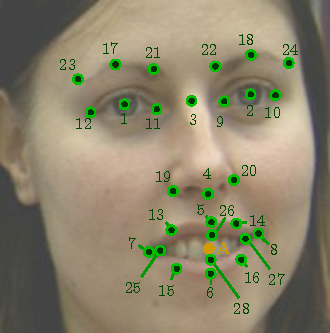
\includegraphics[width = 0.6 \columnwidth]{nvcclass/HeuristicTrackers.pdf}
\caption{Illustration of position of LP Trackers used in the extraction of Heuristic Geometric Features.}
\label{FigureHeuristicTrackers}
\end{figure}

\begin{table}
\centering
\caption{Inter-Culture Correlation of Various Mean Filtered Culture Responses.}
\begin{tabular}{ | c | c | }
\hline
Heuristic & El Kaliouby and Robinson \\
Features & Features \cite{Kaliouby2005}\\
\hline
\hline
Head yaw & Head yaw \\
Head pitch & Head pitch \\
Head roll & Head roll\\
Eyebrow raise & Eyebrow raise\\
Lip pull & Lip pull\\
Lips part & Lip pucker \\
Eye horizontal position (Right) & Lips part \\
Eye horizontal position (Left) & Jaw drop \\
Eye horizontal position (Mean) & Teeth visible \\
Eye vertical position (Right)  & \\
Eye vertical position (Left) & \\
Eye vertical position (Mean) & \\
\hline
\end{tabular}
\label{TableHeuristicFeaturesComparison}
\end{table}

\begin{table}[tb]
\centering
\caption[Heuristic geometric features used to extract facial expression while being robust to pose.]{Heuristic geometric features used to extract facial expression while being robust to pose. Position $A$ is the average position of the outer mouth trackers. $\timeOffset$ is the current frame number. These features were inspired by el Kaliouby and Robinson \cite{Kaliouby2005}.}
\begin{tabular}{ l l }
Head yaw & $\frac{\overline{\rawTracking_{9} \rawTracking_{10}}}{\overline{\rawTracking_{11} \rawTracking_{12}}}$ \\
Head pitch & $\rawTracking_{4}[\timeOffset] - \rawTracking_{4}[\timeOffset-1]$\\
Head roll & $\angle \rawTracking_{9} \rawTracking_{11}$\\
Eyebrow raise & $\frac{(\overline{\rawTracking_{11}\rawTracking_{21}}+\overline{\rawTracking_{1}\rawTracking_{17}}+\overline{\rawTracking_{12}\rawTracking_{23}})_{t}}{(\overline{\rawTracking_{11}\rawTracking_{21}}+\overline{\rawTracking_{1}\rawTracking_{17}}+\overline{\rawTracking_{12}\rawTracking_{23}})_{0}}$\\
Lip pull/pucker & $\frac{(\overline{A\rawTracking_{7}}+\overline{A\rawTracking_{8}})_{t}-(\overline{A\rawTracking_{7}}+\overline{A\rawTracking_{8}})_{0}}{(\overline{A\rawTracking_{7}}+\overline{A\rawTracking_{8}})_{0}}$ \\
Lips part & $\overline{\rawTracking_{26} \rawTracking_{28}} \cdot \overline{\rawTracking_{25} \rawTracking_{27}}$ \\
Right eye horizontal & $\frac{\rawTracking_{11}\rawTracking_{12}\cdot \rawTracking_{11}\rawTracking_{1}}{|\rawTracking_{11}\rawTracking_{12}|}$\\
Left eye horizontal & $\frac{\rawTracking_{9}\rawTracking_{10}\cdot \rawTracking_{9}\rawTracking_{2}}{|\rawTracking_{9}\rawTracking_{10}|}$\\
Mean eye horizontal & $\frac{(\rawTracking_{11}\rawTracking_{12}\cdot \rawTracking_{11}\rawTracking_{1}) (\rawTracking_{9}\rawTracking_{10}\cdot \rawTracking_{9}\rawTracking_{2})}{2|\rawTracking_{11}\rawTracking_{12}||\rawTracking_{9}\rawTracking_{10}|}$\\
Right eye vertical & $\frac{|\rawTracking_{11}\rawTracking_{12}\times \rawTracking_{11}\rawTracking_{1}|}{|\rawTracking_{11}\rawTracking_{12}|}$ \\
Left eye vertical & $\frac{|\rawTracking_{11}\rawTracking_{12}\times \rawTracking_{11}\rawTracking_{1}|}{|\rawTracking_{11}\rawTracking_{12}|}$ \\
Mean eye vertical & $\frac{|\rawTracking_{11}\rawTracking_{12}\times \rawTracking_{11}\rawTracking_{1}| |\rawTracking_{11}\rawTracking_{12}\times \rawTracking_{11}\rawTracking_{1}|}{2|\rawTracking_{11}\rawTracking_{12}||\rawTracking_{11}\rawTracking_{12}|}$\\
Mouth centre & $A=\overline{[\rawTracking_{5},\rawTracking_{6},\rawTracking_{7},\rawTracking_{8},\rawTracking_{13},\rawTracking_{14},\rawTracking_{15},\rawTracking_{16}]}$
\end{tabular}
\label{GeometryFeaturesTable}
\end{table}

Heuristic features focus on only a subset of facial deformations. The next section describes a method to encoding a broader range of face deformations.

\subsection{Algorithmic Geometric Features}
\label{SectionGenerateAlgorithmic}

Manually engineered features encode a subset of facial deformations that are thought to be relevant by their designer. An alternative is to comprehensively encode the shape information of the facial feature trackers. 
%It may also be advantageous for each feature component to correspond to a local area of the face. 
Frame features are exhaustively generated based on a simple geometric measure. This approach is referred to as algorithmic geometric features, abbreviated to \textit{geometric-a}. Ideally, this would encode information pertaining to local deformations of the face in separate features than motion due to head pose changes. Simple distances between pairs of trackers are used (see Figure \ref{FigureAlgorithmicFeatures}), in a similar fashion to Valstar \etal \cite{Valstar2006}. The length of the feature vector $\frameFeature_{geometric-a}$, for $\numTrackers$ trackers, is triangular number $T_{\numTrackers}$ where $T_{\numTrackers} = \frac{\numTrackers(\numTrackers+1)}{2}$. In this work, $\numTrackers=46$ trackers are used to generate algorithmic features (see Figure \ref{FigureTrackerPositions}), therefore $\frameFeature_{geometric-a} \in \mathbb{R}^{T_{46}}=\mathbb{R}^{1035}$. For two trackers of index $a \in \mathbb{R}$ and $b \in \{0...\numTrackers\}$, where $1 \le a < b$, the distance is computed:

\begin{gather}
\frameFeature_{unnormalised\_alg}^{a + b + T_{b-1}} = |\rawTracking_{a} - \rawTracking_{b}|
\end{gather}

%Algorithmic features are simple to calculate and encode a wide range of facial deformations but they tend to include a large proportion of redundant information. Also, beyond a reasonable number of trackers, the feature length may become excessive. Geometric distance pairs are robust to some forms of head pose changes. The head pose is indirectly encoded by calculating the distances between pairs of rigid points on the face. Algorithmic features encode information from a local area of the face, except when the motion is entirely due to changes in head pose. 
Although these feature components encode shape information from localised areas of the face, the features tend to include redundant information and are not robust to scale changes.

\thesiscomment{DISCUSS Algorithmic features of \cite{Pantic2006} but they only use one reference point and discretised the result}

\thesiscomment{IDEA: Discuss which types of head rotations do not change feature?}

\thesiscomment{TODO: Do I have a correct understanding of ``appearance''? Does it depend on the pose of the object?}

\begin{figure}[tb]
\centering
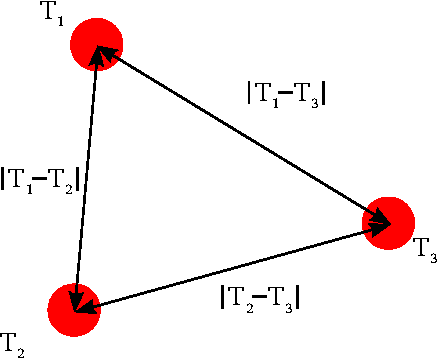
\includegraphics[width = 0.5 \columnwidth]{nvcclass/algorithmic-features.pdf}
\caption{A trivial example of how algorithmic geometric features are calculated for 3 tracked points. Exhaustive distance pairs of trackers are calculated. \thesiscomment{MathInFig}}
\label{FigureAlgorithmicFeatures}
\end{figure}

%The appearance and shape of a face is determined by several factors, including facial displays, illumination, age, gender, glasses, cosmetics, facial hair, head pose and identity. Also, people vary in how far facial points move during a facial display. For example, a head that is physically larger would often have facial points moving a larger distance during a smile, when compared to a smaller head. Feature generation, as described in the previous section, can partly remove or separate the effect of head pose from local deformations caused by facial displays. However the effect of identity can be significant and to make comparisons between different people, differences caused by identity need to be removed as far as practically possible.

%The way people express emotions and \ac{NVC} varies between individuals (see Section \ref{BackgroundPeopleVaryInExpression}). If these identity based effects differ in our features by a simple difference in scaling of features, it may be possible to remove this effect using simple techniques. For example, if someone moves further when nodding in agreement than another person, the features can be rescaled to ensure this corresponding behaviour is equivalent. However, differences in the timing of facial displays between individuals are not as simple to normalise. 
The features are then processed to reduce the effect of identity. This normalisation is not applied to the other types of features (see Figure \ref{FigureClassificationOverview}), although later chapters have normalisation applied in a consistent fashion to avoid this problem. Each feature component is rescaled and zero centred. This removes shape information due to both identity and some types of expressivity by removing person specific differences in facial deformation magnitude. Information that relates to facial shape deformation, in terms of a difference from the average face, is retained. For a video sequence of $\numSeqFrames$ frames, all frame feature vectors are concatenated into a frame feature matrix $\frameFeatureMatrix \in \mathbb{R}^{1035 \times \numSeqFrames}, \numSeqFrames \in \mathbb{N}$. The mean $\componentMean$ and variance $\componentVariance$ values of each feature component are used to normalise and zero centre the feature ($\componentVariance, \componentMean \in \mathbb{R}^{1035}, i \in \{0...1035\}$, $t \in \{0...\numSeqFrames\}$):

\begin{gather}
\label{EqnFeatureComponentMean}
\componentMean^i = \frac{\displaystyle\sum\limits_{j=0}^{\numSeqFrames}{\frameFeatureMatrix_{unnormalised\_alg}^{i,j}}}{\numSeqFrames} \\
\label{EqnFeatureComponentVar}
\componentVariance^i = \frac{\displaystyle\sum\limits_{j=0}^{\numSeqFrames}{{\frameFeatureMatrix_{unnormalised\_alg}^{i,j}}^2}}{\numSeqFrames} - {\componentMean^i}^2 \\
\label{EqnNormaliseFeatureRange}
\frameFeatureMatrix_{geometric-a}^{i,t} = \frac{\frameFeatureMatrix_{unnormalised\_alg}^{i,t} - \componentMean^i}{\sqrt{\componentVariance^i}}
\end{gather}

$\frameFeatureMatrix_{geometric-a}$ is easy to compute but it requires an existing set of frames covering the range of \ac{NVC} signals to calculate the mean $\componentMean$ and scaling factors $\componentVariance$ used in normalisation. This makes the approach unsuitable for immediate \featureGeneration of a previously unseen face. 
%However, after a training session, the system can learn a new face and this method may be applied. If this is not practical, the method can be simplified to only zero centring the features without scaling, based on a frontal view of the face. Alternatively, a standard face shape can be used to normalise the features but this may not be as effective as a person specific face model.

%Algorithmic features do not completely separate the effect of head pose from local deformations of the face. The following section outlines another feature encoding approach to achieve this.

\subsection{Tracking-based Features using PCA and ICA Dimensionality Reduction}

%Movement in tracker positions are due to both head pose changes and local deformations of the face. Potentially both kinds of  motion may be useful for classification of \ac{NVC}. Broadly speaking, facial expression may be considered equivalent at different poses. A smile with the head pitched back is largely equivalent to a smile with the head pitched forward. 
\ac{PCA} and \ac{ICA} can be used to separate information due to changes in pose from information due to local deformation. This is necessary because raw features from tracking contain translations and other movement information that is not necessarily relevant to \ac{NVC} classification. Directly using raw features would result in poor recognition performance. These dimensionality reduction techniques subdivide a signal by projecting it on to a new set of basis vectors; the basis vectors in the case of \ac{PCA} correspond to a particular overall deformation of the face. \ac{PCA} selects eigenvectors that are the largest orthogonal modes of variation, while \ac{ICA} selects basis vectors that are statistically independent. The use of \ac{PCA} on tracking data has previously been used by Lien \etal \cite{Lien1998}.
%Because the head pose causes large changes in tracker positions, it is typically encoded in the first few \ac{PCA} components. Deformation due to local face deformations are usually encoded in the later \ac{PCA} components. 
The basis eigenvectors are learned in an unsupervised fashion but generally do not correspond to local areas of the face, nor guarantee that they are optimal for recognition.

For $\numTrackers$ trackers, the positions on a single frame is designated as $\rawTracking \in \mathbb{R}^{2 \times \numTrackers}$. For a video of $\numSeqFrames$ frames, the tracking data is reshaped into a $2\numTrackers \times \numSeqFrames$ matrix. This tracking matrix is zero centred to form matrix $\normalisedTracking$. Performing \ac{PCA} on $\normalisedTracking$ produces $2\numTrackers$ principal components. Each frame was then projected on to these basis vectors to form a frame feature $\frameFeature_{pca} \in \mathbb{R}^{2\numTrackers}$. A similar procedure was used to project frames into \ac{ICA} space. Two specific \ac{ICA} implementations were used: FastICA \cite{Hyvarinen1999} and CuBICA \cite{Blaschke2004}. FastICA is advantageous because of its fast convergence, while CuBICA is able to separate asymmetrically distributed sources but at a higher computational cost \cite{Wang05}. The frame feature corresponding to these methods are referred to as $\frameFeature_{fastica}$ and $\frameFeature_{cubica}$ respectively.

%The next two sections describes various approaches to head pose estimation based on tracker positions, which is useful for aligning images, and possibly as another feature suitable for \ac{NVC} recognition.

\subsection{\ac{LMA} Head Pose Estimation}

The shape deformation of the face has been considered, but appearance information may also contribute to \ac{NVC} recognition. For example, the appearance of wrinkles or the teeth cannot be effectively tracked due to their transitory appearance. To make comparisons between different frames and persons, the faces need to be aligned. This enables direct comparison of corresponding positions for the purposes of \ac{NVC} recognition. 

Head pose may be estimated by model fitting and cost minimisation. Cost minimisation is performed by minimising least square errors by \acf{LMA}, and a simple head model based on an average head shape and expressed in homogeneous coordinates ${\headMeshPos} \in \mathbb{R}^{\numTrackers \times 4}$. This is similar to the approach used by Liu and Zhang \cite{Liu2000}, but the head model is simplified to ignore the effect of expression. The model fitting results in estimates for 3 translation components and 3 Euler rotation components. 
%This is concatenated into a frame feature vector of $\frameFeature_{lma}$. 
Because of the simplicity of the model, it cannot encode facial expression but it does encode head pose information in an intuitive way. For example, head nodding and shaking are encoded as two distinct components. For each frame, the head post model error $\modelFitError$ is estimated as follows:

\begin{gather}
\modelFitError(\headRotation,\headTranslation) = \displaystyle\sum_{i=1}^{\numTrackers} { ||{\rawTracking}_{i} - \projFunc(\headRotation \headMeshPos_i + \headTranslation)||^2 }
\label {LmPoseEquation}
\end{gather}

Where $\projFunc$ is the perspective projection function, $\headTranslation$ is the translation (where $\headRotation \in \mathbb{R}^{4 \times 4}$ is the head rotation matrix corresponding to the Euler angles {$\headRotation_{pitch}$, $\headRotation_{roll}$, $\headRotation_{yaw}$} and $\headTranslation \in \mathbb{R}^{4}$ is the head translation $\headTranslation=\{\headTranslation_x, \headTranslation_y, \headTranslation_z, 1.\}$). The pose parameters are varied to find the minimum model fit error. The pose variables $\headRotation_{pitch}$, $\headRotation_{roll}$, $\headRotation_{yaw}$ and $\headTranslation_x, \headTranslation_y, \headTranslation_z$ are concatenated to form a frame feature $\frameFeature_{lma} \in \mathbb{R}^{6}$.

%Model fitting can range from simple approaches to complex and computationally intensive. The following section describes a simple head pose estimation method that can also be applied to image alignment.

\subsection{Affine Head Pose Estimation}

\begin{figure}[tb]
\centering
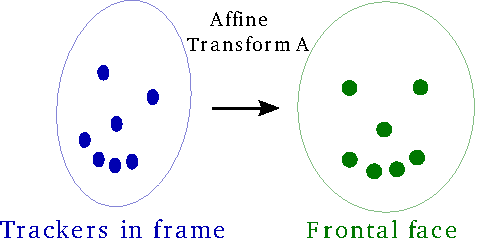
\includegraphics[width = 0.5 \columnwidth]{nvcclass/affine-transform.pdf}
\caption{An affine transform is calculated to transform the current face on to the frontal face shape. This diagram has been simplified to only use 7 tracked features. \thesiscomment{MathInFig}}
\label{FigureAffineHeadPose}
\end{figure}

%Head pose estimation is maps a specific head pose into a specific point in feature space. It is desirable that the feature space is something that can be intuitively understood but this is not strictly necessary. 
If the tracking positions $\rawTracking$ are re-expressed as the homogeneous coordinate matrix ${\rawTrackingHomog} \in \mathbb{R}^{\numTrackers \times 3}$, an affine transform of tracker positions $\rawTrackingHomog$ to another frontal reference shape $\rawTrackingHomog'$ encodes the head pose.
%Of course a human head, being a {3D} object, cannot be exactly transformed to frontal pose by an affine transform but despite this, the head pose is encoded in a form usable for classification. 
The affine transform can also be used to align the face, but the affine transform approximation breaks down as the face rotates away from the frontal view.
The affine transform $\approxaffine \in \mathbb{R} ^ {3 \times 3}$ can be estimated by taking the matrix Moore-Penrose pseudo-inverse ($\rawTrackingHomog^{+}$) as shown in Equation \ref{AffineEquation}. The result can be reshaped to a frame vector vector $\frameFeature_{affine} \in \mathbb{R} ^ {6}$.

\begin{gather}
\rawTrackingHomog' = \approxaffine \cdot \rawTrackingHomog \\
\approxaffine = \rawTrackingHomog' \cdot \rawTrackingHomog^{+}
\label {AffineEquation}
\end{gather}

%The previous sections have described how facial deformations and head pose changes are encoded into frame based features. The next section describes how facial appearance can be encoded.

\subsection{Uniform Local Binary Patterns}

%Certain facial displays are based on appearance changes in the face with little or no significant deformation of the face shape. For example the appearance of a cheek pucker or reddening of the face in blushing. Tracking features are poor at encoding appearance changes, since they only correspond to facial feature positions. 
There are many possible approaches to encoding facial texture (see Section \ref{BackgroundEncodeFacialInfo} for background). \acf{LBP} \cite{Ojala2002} is used in this work, because it has been shown to be effective in encoding facial texture for emotion recognition \cite{Shan2009}. \ac{LBP} focuses on encoding texture information, often in grey-scale images. The role of colour is not considered in this work, because \ac{NVC} based facial colour changes are relatively rare and are a subtle effect. Local binary patterns are based on comparisons between a central pixel intensity and the intensities of nearby pixels. The comparison is a single ``greater than'' or ``less than or equal'' binary choice. The local pixels are often arranged in a simple pattern, such as a circle or a series of concentric circles. In this work, the simplest \ac{LBP} operator is used, which considers the eight pixels surrounding a central pixel (see Figure \ref{FigureLbp}), denoted as $LBP_{(8,1)}$. Each combination of possible binary intensities is mapped into a code book. \ac{LBP}s in a region of interest are then usually used to form a histogram of code words. Ojala \etal \cite{Ojala2002} focused on \ac{LBP}s that have, at most, two bitwise transition in the circle of pixels, which they termed ``uniform''. These histogram features were found to be effective, while reducing the number of code words from 256 to 59. The histograms are normalised to remove the effect of the number of \ac{LBP} samples. These histograms may be used as features for recognition. \ac{LBP}s are computationally simple and are largely robust to illumination changes, because of the removal of the absolute difference intensity information. For the image intensity of eight pixels $f_i \in \mathbb{R} ^ {8}, i = \{0...7\}$ surround central pixel $f_c \in \mathbb{R}$, the pixel comparison vector $\lpbWord \in \mathbb{Z} ^ {8}$ and \ac{LBP} value $LBP_{(8,1)} \in \mathbb{Z}$ is computed as:

\begin{gather}
\lpbWord(f_i-f_c) = \begin{cases} 1, & f_i \ge f_c \\ 0, & otherwise \end{cases}\\
\diffblock{LBP_{(8,1)} = \displaystyle\sum\limits_{j=0}^7 \lpbWord(f_j - f_c)2^P}
\end{gather}

\begin{figure}[tb]
\centering
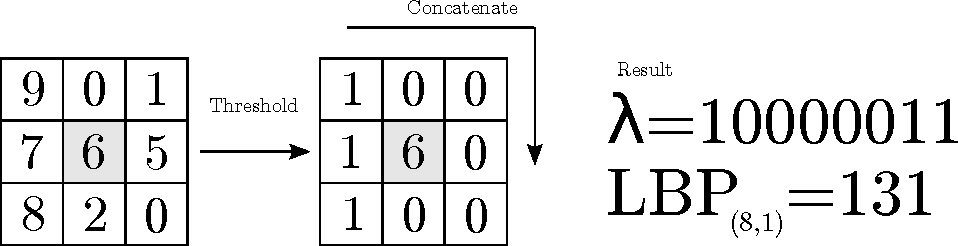
\includegraphics[width = 0.8 \columnwidth]{nvcclass/lbpfigure.pdf}
\caption{The basic $LBP{(8,1)}$ operator. For each pixel, the adjacent pixels $f_i$ are thresholded $\lpbWord$ and concatenated to form an \ac{LBP} code.}
\label{FigureLbp}
\end{figure}


The face region was subdivided into a grid of $\lbpgridwidth$ by $\lbpgridheight$ rectangles (similar to Feng \etal \cite{Feng2005}, $\lbpgridwidth, \lbpgridheight \in \mathbb{N}$). The grid used the affine transform $\approxaffine$, described in the previous section, to maintain the alignment with the underlying facial features. Uniform \ac{LBP}s were calculated on each rectangle in the grid, producing $\lbpgridwidth\times\lbpgridheight$ histograms. These histograms were concatenated into a frame feature vector $\frameFeature_{lbp} \in \mathbb{R} ^ {59\cdot\lbpgridwidth\cdot\lbpgridheight}$.

\begin{figure}[tb]
\centering
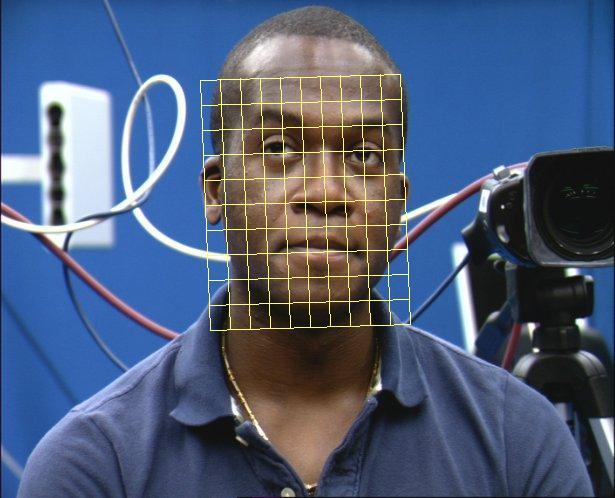
\includegraphics[width = 0.8 \columnwidth]{nvcclass/lbp-face-grid-overlay.jpg}
\caption{Histograms of \ac{LBP} value frequencies are calculated within each area of a $\lbpgridwidth\times\lbpgridheight$ grid. The grid is aligned to the face using an affine transform which reduces the effect of head pose and translation.}
\label{FigureLbpGrid}
\end{figure}

%The face alignment is carried out using an affine transform, but the affine assumption breaks down at extreme non-frontal head poses. If the face alignment is poor, the grided areas will not necessarily have a correspondence with other face samples. This would manifest itself as noisy features which are unsuitable for recognition. This may be avoided by using more sophisticated approaches to face alignment but these are not considered in this work.

%The features described in this section are used to encode shape and appearance of the face. However, face shape and appearance varies between people. The next section returns to discussing automatic classification of \ac{NVC}.

\section{Classification for \ac{NVC}}
\label{SectionClassificationMethods}

%Human behaviour is highly variable with little direct relationship between simplistic features and the \ac{NVC} labels. This can partly be addressed by the use of a broader range of features. 
%The \featureGeneration methods employed have been described in Section \ref{SectionFeatureGeneration}. 
%However, it can be difficult to manually determine which features are relevant and how they should be combined to predict a label for a test clip. Fortunately, this is not necessary because there are many automatic classification methods available, as Section \ref{BackgroundSupervisedClassification}. 
The automatic \ac{NVC} system was tested using both Adaboost and \ac{SVM} classifiers. These classifiers have been shown to be effective in various facial analysis applications. They are both binary classifiers, which are suitable for our constrained problem. The method for comparing the classifier predictions to ground truth is described in Section \ref{SectionClassificationPerformance}. The \ac{NVC} corpus contains video clips of different lengths but temporal variations are not directly modelled by these classifiers. The approach used here is to classify each frame and then fuse the classifier outputs to produce a final label. 
%Without modelling the temporal variations for each class, the classifier model is relatively simple. 
Basic temporal models that encode information from multiple frames are used in Sections \ref{SectionTemporalFeatures} and \ref{SectionClipFeatureExtraction}. The training samples used to create the classifier model corresponding to individual frames, however not every frame necessarily contains relevant information. A training clip is used in its entirety, which can lead to a proportion of irrelevant frames being included in the classification model, resulting in a drop in performance. 
%Therefore, the training data is relatively noisy. 
%The frames for clips are concatenated into a 2{D} matrix for the purposes of training and testing. 
For a clip of length $\numClipFrames$ frames, the $\numFeatures$-dimensional frame features $\frameFeature$ are concatenated into a clip feature matrix $\clipFeature \in \mathbb{R}^{\numClipFrames \times \numFeatures}$. All clip feature matrices $\clipFeature$ are concatenated into a global feature vector $\globalFeature$, which for a corpus of $\framesInCorpus$ frames: $\globalFeature \in \mathbb{R}^{\framesInCorpus \times \numFeatures}$.

%The two classifiers used in the comparison will now be examined in more depth.

\subsection{Adaboost Classifier}
\label{SectionAdaboost}

Adaboost is a supervised binary classifier based on a weighted combination of an ensemble of ``weak learner'' binary inputs \cite{Freund1996}. The input data can contain significant feature noise, but as long as the features are better than random, they are combined by Adaboost to produce a strong classifier. The algorithm operates by incrementally adding feature components to a bank with a corresponding weight. The algorithm selects feature components in an attempt to reduce the training error while focusing on samples that are hardest to classify. At termination, the selected features and weights specify a strong classifier that may be used to predict unseen examples. 

Adaboost is simple to implement, computationally efficient, generally avoids over-training and provides explicit information as to which features are relevant. However, it does not perform as well as other machine learning techniques in some situations. Mislabelled training data can be problematic for some types of classifier, such as Adaboost \cite{Natsuki2008}.

All the \featureGeneration techniques described in Section \ref{SectionFeatureGeneration} result in continuous value features. However, Adaboost is limited to binary input data and two class problems. 
%Continuous variables are discretised into a suitable input format for Adaboost but this may result in information loss. 
For each continuous value feature component, the discretisation is performed by $\numThresholds$ binary thresholds, designated as $\thresholdVal \in \mathbb{R}^{\numThresholds \times \numFeatures}$. The placement of thresholds for feature component $j  \in \{1...\numFeatures\}$ is determined as follows ($i \in \{1...\numThresholds\}$):

\begin{gather}
\thresholdVal_{1,j} = \overline{\globalFeature_j} - \sigma(\globalFeature_j) \\
\thresholdVal_{\numThresholds,j} = \overline{\globalFeature_j} + \sigma(\globalFeature_j) \\
\thresholdVal_{i,j} = \frac{i-1}{\numThresholds-1}(\thresholdVal_{\numThresholds,j} - \thresholdVal_{1,j}) + \thresholdVal_{1,j}
\end{gather}

where $\globalFeature_j$ is the $j$th row of the global feature matrix $\globalFeature$ and $\overline{\globalFeature_j}$ is the mean of $\globalFeature_j$ and $\sigma(\globalFeature_j)$ is the variance of the $j$th feature component. A scaling factor of one standard deviation was experimentally determined. The thresholds are computed on all video samples, which arguably violates the separation of training and test data (\ac{SVM}s, presented in the next section, do not have this issue.) However, this effect should be minimal because little person specific information is used. These thresholds are then applied to the feature vector to produce a discretised feature vector $\discretisedFeatures \in \mathbb{R}^{\numClipFrames \times \numFeatures\ \numThresholds}$, $a \in {1...\numClipFrames}$:

\begin{gather}
\discretisedFeatures_{a,\numThresholds (j-1)+i} = \begin{cases}
+1, & \mbox{if } \clipFeature_{a,i} \ge \thresholdVal_{j,i} \\ -1, & \mbox{if } \clipFeature_{a,i} < \thresholdVal_{j,i}
\end{cases}
\end{gather}

%
%
These thresholds effectively subdivide the feature space by axis parallel hyperplanes with the middle hyperplane positioned on the mean value. %The automatic system was also evaluated using a second machine learning technique called \ac{SVM}, which is discussed in the next section.

\subsection{Support Vector Machines Classifier}
\label{SectionSupportVectorMachines}

An \ac{SVM} is a supervised learning method originally formulated for binary classification \cite{Cortes1995, Vapnik1998}, although an extension to regression \cite{Drucker1997} also exists. \ac{SVM}s use the concept that, although in an original feature space the training samples may not be linearly separable, there exists a non-linear mapping to another space in which a problem is linearly separable. The space is remapped by the use of kernels centred on training samples. An unseen test sample is transformed into this new space and classified based on a simple threshold. The algorithm is difficult to implement efficiently but allows continuous value input variables. This avoids the need to discretise our input features. Unfortunately, the algorithm provides no direct way to examine which features are relevant. This chapter uses the original ``C-SVM'' formulation of \ac{SVM}s, rather than the later $\nu$-SVM variant \cite{Scholkopf2000}. An \ac{SVM} may be trained with various kernels; in this study the \ac{RBF} kernel is used, which is often seen to be effective \cite{Shan2009}. A regression variant of \ac{SVM}, called $\nu$-SVR, is used in Chapter \ref{ChapterNvcRegression}.

\thesiscomment{CHECK we are really using C-SVM}

\section{NVC Labels and Use of Clear Examples in Classification}
\label{SectionClearExamples}

%This section discusses how a problem suitable for supervised learning has been framed, based on the annotation data discussed in the previous chapter. Many supervised learning problems are based on having a single value label per sample (see Section \ref{BackgroundFramingClassificationProblem}). However, t
The annotation questionnaire was based on four independently varying \ac{NVC} signals. %The average rating for a video clip can be represented as a point in a 4{D} continuous space. 
%This multi-dimensional sample label is similar to other approaches that encoding emotion in a 2{D} space such as Arousal and Valence \cite{Nicolaou2011}\cite{Wollmer2009}, or Active/Passive and Positive/Negative \cite{Cowie2000}. Although it is possible to use dimensional reduction techniques or clustering to reduce the label space but this may lead to a loss of label information. These studies treat each label as an independent problem to be solved. 
%Performance for each label category is quoted as a separate figure. In the context of supervised learning, these approaches may be considered as a vector sample label which is an extension to a common single value label supervised learning. However, it is currently unknown if \ac{NVC} can be accurately and conveniently encoded an a low dimensional space. Therefore, I use the four separate \ac{NVC} signal ratings as a 4 component sample label. 
The four components of \ac{NVC} rating categories are four independent problems to be solved.
Predictions that distinguish between strong and weak intensity signals, rather than simply positive and negative classification, makes the prediction labels richer and possibly more useful for real applications. However, many machine learning techniques only address classification problems. Also, given the expected difficulty in completely solving the \ac{NVC} recognition problem (see Section \ref{BackgroundWhyIsNvcDifficult}), this chapter addresses a simpler problem by reducing it to a classification task. This is similar to existing studies conducted on emotion recognition that treated the task as a two class \cite{Rosenblum1996} or multi-class problem \cite{Cohen2000}. The problem of directly recognizing different \ac{NVC} intensities is addressed in Chapter \ref{ChapterNvcRegression}. A set containing all clips in the corpus is designated as $\allClipSet$. As discussed in Section \ref{SectionAnalysisOfMeanRatings}, the consensus mean rating of a clip is denoted $\clipConcensus$ and contains 4 components corresponding to the four \ac{NVC} signals.

In this study, clips that were rated as strongly showing an \ac{NVC} signal were assigned to first positive set and examples that had been rated (by consensus $\clipConcensus$) as an absence of an \ac{NVC} signal were assigned to the negative set. Only the 25 highest and 25 lowest ratings were considered as clear examples, as this was judged to be enough for training while excluding more difficult ambiguous examples from both training and testing. Because each component of $\clipConcensus$ can vary independently, the clip sets containing positive and negative examples of \textit{thinking} are different to the positive and negative sets for \textit{agree}. The clear examples for each \ac{NVC} category are designated as follows: positive \textit{thinking} set $\clearClipSet^{+}_{thinking}$, negative \textit{thinking} set $\clearClipSet^{-}_{thinking}$, positive \textit{agree} set $\clearClipSet^{+}_{agree}$, negative \textit{agree} set $\clearClipSet^{-}_{agree}$, etc. ($\clearClipSet^{+}_{\nvcCategory} \in \allClipSet, \clearClipSet^{-}_{\nvcCategory} \in \allClipSet$) The clips are ordered based on the mean annotator rating, $\nvcCategory \in \setCategories$:

\begin{gather}
 \overline{\allClipSet}_{\nvcCategory} = \{i \in \{1,...,\numClips\} : \clipConcensus_{\nvcCategory,i} \le \clipConcensus_{\nvcCategory,i+1} \}
\end{gather}

The indices of the 25 most positive and 25 most negative clips are identified:

\begin{gather}
 \overline{\allClipSet}^{+}_{\nvcCategory} = (\overline{\allClipSet}_{\nvcCategory,i})^{\numClips}_{i=\numClips-25} \\
 \overline{\allClipSet}^{-}_{\nvcCategory} = (\overline{\allClipSet}_{\nvcCategory,i})^{25}_{i=1}
\end{gather}

The final positive and negative sets are then established:

\begin{gather}
 \clearClipSet^{+}_{\nvcCategory} = \{\allClipSet_i : i \in \overline{\allClipSet}^{+}_{\nvcCategory}\} \\
 \clearClipSet^{-}_{\nvcCategory} = \{\allClipSet_i : i \in \overline{\allClipSet}^{-}_{\nvcCategory}\}
\end{gather}

%Simplifying the problem to binary classification by discarding intermediate rated clips makes our problem comparable to other research studies in emotion recognition that have used acted emotions which tend to produce high intensity examples. But in contrast to precious acted studies, natural conversations are used in this thesis. With insights gained in this sub-problem, Chapter \ref{ChapterNvcRegression} considers regression analysis of the entire set of clips.

%\begin{figure}
%\centering
%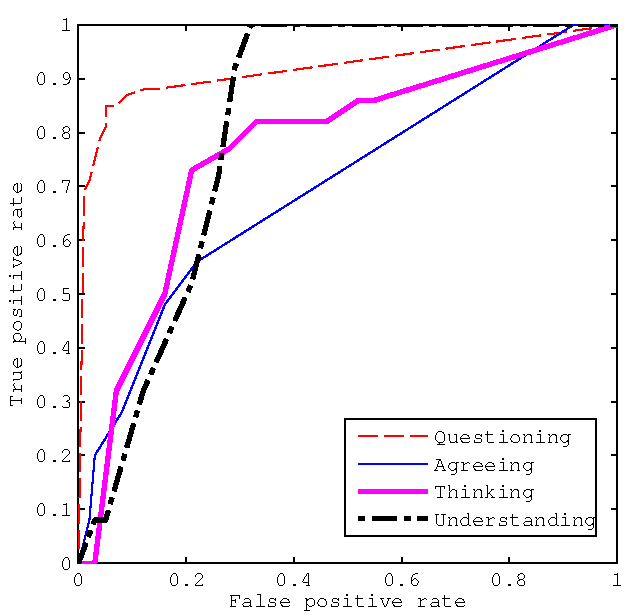
\includegraphics[width = 0.6 \columnwidth]{nvcclass/HumanRoc.pdf}
%\caption{An \ac{ROC} plot of human rating ratings of clear \ac{NVC} examples, compared to a ground truth based on human consensus annotations. Consensus is highest for \textit{question} and lowest for \textit{agree}.}
%\label{FigureHumanClassificationPerformance}
%\end{figure}

%Individual annotators consistency with a clip's positive and negative set membership ($\clearClipSet$) can be determined. This builds upon the inter-annotator analysis in Section \ref{SectionAnalysisOfMeanRatings}, but the binary classification property is used to perform a \ac{ROC} analysis. 
For a single \ac{NVC} signal category $\nvcCategory$, the union between positive and negative sets is then determined for each \ac{NVC} signal $\clearClipSet^{clear}_{\nvcCategory} = \clearClipSet^{+}_{\nvcCategory} \cup \clearClipSet^{-}_{\nvcCategory}$. There were only a few examples of \ac{NVC} disagreement and the three other \ac{NVC} signals had rating scales from neutral to intense expression. For these reasons, examples of disagreement were discarded and \textit{agree} samples were drawn from neutral and positive samples. The next section describes how these machine learning methods are evaluated and compared.

\section{Performance Evaluation Methods for Variable Length Video Clips}
\label{SectionClassificationPerformance}

%The automatic system is trained on features generated from examples of positive or negative \ac{NVC} signals. 
%The machine learning methods used by the automatic systems, either Adaboost or \ac{SVM}, was discussed in the previous section. 
%After training an Adaboost or \ac{SVM} model, the automatic system can make a prediction as what what \ac{NVC} signals are present in an unseen video clips. However, different approaches have different levels of performance. This section discusses how the performance of an automatic system can be assessed.

%\begin{figure}[tb]
%\centering
%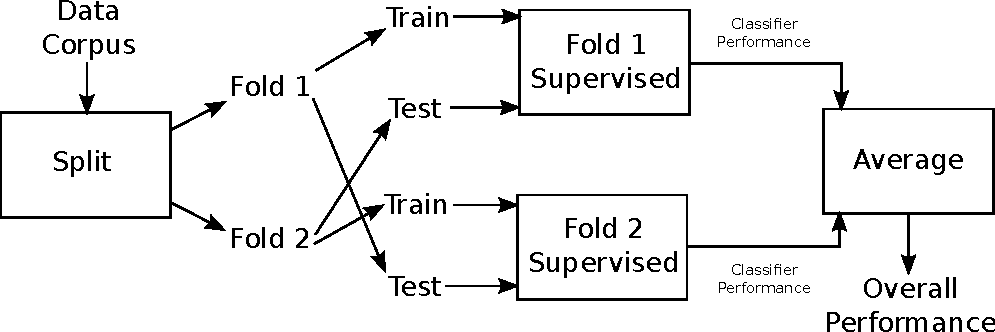
\includegraphics[width = 0.9 \columnwidth]{nvcclass/crossvalSystem.pdf}
%\caption{Overview of two fold Cross validation split of data. The performance from each fold is combined to compute an overall performance. The test results in this chapter are actually performed using eight fold cross validation, two fold is used in this figure as a simplified illustration of the concept.}
%\label{FigureCrossVal}
%\end{figure}

Given the relative difficulty in collecting and annotating data, the available data should be used as efficiently as possible. Therefore, cross validation testing is used, which tests an automatic system in multiple folds. Each fold uses a different partitioning of the data into sets of training and test samples.
%In this thesis, ``unseen data'' is synonymous with ``test data''. 
%The seen data is used to train an automatic system, while the unseen data is reserved for performance evaluation of a system. 
%Cross validation is preferable to using a single partition of the data because it is expected that person dependent expression of \ac{NVC} will make the unseen data in each fold quite different. To achieve a stable performance score, it would be advantageous to have every subject appear in the test data during one of the cross validation folds. 
Eight fold cross validation is used in both person dependent and person independent tests. For person independent testing, this is equivalent to ``leave one subject out'' testing. 
%Using a higher number of folds increases the size of the training set. However, using a larger number of folds has higher computational resources requirements.

%Performance of automatic systems can be measured using various statistical metrics, with each having a different emphasis. These include precision, recall, robustness and area of applicability (Sokolova \etal \cite{Sokolova2006}). This chapter is concerned with binary classification, the discussion will focus on techniques that specialise in this task. In contrast, regression performance metrics are discussed in Section \ref{SectionRegressionAndPerformanceEvaluation}. Perhaps the most widely used binary classification metrics are accuracy, F1 score and the area under an \ac{ROC} curve (defined in Equations \ref{EquationFirstBinaryMetric} to \ref{EquationLastBinaryMetric}). Given an unseen test sample, binary classifiers can predict a label and many classifiers also are capable of providing a prediction confidence score. Without a well defined application to inform the selection criteria for the performance metric, the one with the most sensitivity to prediction confidence was thought be the best selection: area under \ac{ROC} curve.

\thesiscomment{DISCUSS positive and negative are balanced which appropriate for ROC}

The sample videos have various lengths and the automatic system needs to process them in a way that enables comparison with the true label.
The difference between the predicted labels and actual labels is then quantified. Perhaps the most widely used binary classification metrics are accuracy, F1 score and \ac{ROC} \ac{AUC}. Apart from being a popular metric, \ac{ROC} analysis is used because the application and acceptable rate of failure are unknown. \ac{ROC} analysis shows the system behaviour under a range of false positive rates. 
%\ac{ROC} analysis is used because it enables results in this section to be compared to automatic classification systems in Section \ref{SectionClassificationPerformance}. 
The equations for the commonly used metrics are (adapted from \cite{Sokolova2006}): 

\begin{gather}
\label{EquationFirstBinaryMetric}
positive = true\_positive + false\_negative \\
negative = true\_negative + false\_positive \\
accuracy = \frac{true\_positive + true\_negative}{positive + negative}\\
precision = \frac{true\_positive}{true\_positive + false\_positive}\\
recall = \frac{true\_positive}{positive}\\
f1\_score = \frac{2 \cdot precision \cdot recall}{precision + recall}
\end{gather}

Computing the \ac{AUC} of \ac{ROC} requires a sweep of a decision threshold to determine the false positive ($fpr$) and true positive rates ($tpr$). This is often intuitively understood as the area under a plot of $tpr$ vs. $fpr$, but can also be expressed mathematically as:

\begin{gather}
fpr=\frac{false\_positive(threshold)}{negative} \\
tpr=\frac{true\_positive(threshold)}{positive} \\
\label{EquationLastBinaryMetric}
area\_under\_roc=\int_0^1 trp(fpr)\,\mathrm{d}fpr
\end{gather}

%To provide a baseline of human performance in \ac{NVC} recognition, the level of agreement of annotators with the consensus score can be quantified. For $\numAnnotators$ annotators, an annotator $i \in \{0..\numAnnotators\}$ predictions $\singleAnnotatorRatings_{i, \nvcCategory} = \{\ratingOfClip_j: (\ratingOfClip_j, \annotatorOfRating_j) \in \rawAnnotation_{\nvcCategory,\clipId}, \clipId \in \clearClipSet^{clear}_{\nvcCategory}, \annotatorOfRating_j=i\} \in \mathbb{R}^{\numAnnotators \times 4}$ are compared to the consensus rating based on all other annotators $\clipConcensus(\{\ratingOfClip_j: (\ratingOfClip_j, \annotatorOfRating_j) \in \rawAnnotation_{\nvcCategory,\clipId}, \clipId \in \clearClipSet^{clear}_{\nvcCategory}, \annotatorOfRating_j \ne i\})$. 
%$\clipConcensus(\rawAnnotation \texttt{\char`\\} \rawAnnotation^i)$
%For each clip $\clipId \in \clearClipSet^{clear}_{\nvcCategory}$, a moving threshold can be applied to the individual ratings set $\rawAnnotation^{\clipId}_{\nvcCategory}$ to provide sets of binary predictions. These are compared to the clip label, which is true if $\clipId \in \clearClipSet^{+}_{\nvcCategory}$, otherwise false. 
%This is used to form an \ac{ROC} curve of human performance in Figure \ref{FigureHumanClassificationPerformance} (\ac{AUC}: \textit{agree} $0.70$, \textit{thinking} $0.77$, \textit{understand} $0.82$ and \textit{question} $0.92$). As expected, human performance is well above chance classification. Humans are most consistent in identifying clear examples of \textit{question} but are least consistent for \textit{agree}. 
%Questions may be easy for humans to identify because they are almost always accompanied by clear audio cues (word usage and voice prosody), and asking a question is usually a binary action with no concept of a ``half questioning'' state, unlike the quite plausible cases of ``half agreeing'' and ``half understanding''. The other \ac{NVC} signals may be comparatively harder to recognise as they rely on ambiguous visual information and are dependent to \ac{NVC} context (see Section \ref{BackgroundWhatFactorsInfluenceNvc}). Another way of interpreting Figure \ref{FigureHumanClassificationPerformance} is to consider that disagreements in ratings presumably have a causal basis. However this implies a violation of our initial assumption that our annotator group is homogeneous. Our annotators are generally in agreement, although there is some evidence of minor variation in their annotation responses. 
%Further work into reducing inter-annotator agreement may be beneficial in understanding this issue (building on the work of Reidsma \etal \cite{Reidsma2008}).

%Prediction confidence scores should also be used, to make the performance metric more sensitive to small changes. 
Given a two class problem, there are a few different approaches to process a variable length clip to enable comparison with the true label:

\begin{itemize}
 \item For each frame in a test clip, the classifier makes a binary prediction. The proportion of positive predictions is taken as the overall positive confidence score. 
 %This is a form of decision level fusion. 
 This method is referred to as ``clip level'' testing. This classification of individual video clips is distinct from event recognition, which is the detection of limited duration events in a longer video \cite{Jiang2012}.
 \item For each frame, calculate the confidence that the frame is positive. The predictions from multiple frames forms a set of predictions. This set is converted to multiple sets of binary predictions using a  moving threshold, as done with a standard \ac{ROC} analysis. Each thresholded binary prediction is then compared to the video clip label. This side steps the need for fusion and is referred to as ``frame level'' testing.
 \item Combine the frames to form an overall clip feature vector of fixed length. This concept is explored in Section \ref{SectionDigestVector}.
 \item Use a machine learning method that is dedicated to sequence classification or \ac{MIL} classification. This is discussed further in Section \ref{SectionHmm}. %In our unpublished initial tests using \ac{MIL}, no significant improvement in performance was observed by using \ac{MIL}. This may be because of the high variability in \ac{NVC} expression (further discussed in Section \ref{SectionVisualisingGaze}).
\end{itemize}

The first two approaches are used to evaluate performance. They were selected because they both utilise confidence ratings which may be evaluated by an \ac{ROC} curve. %Our labels are based on annotation of a complete clip, and this is directly tested by clip level evaluation.

%Given that cross validation testing is used, there are different approaches on how data is assigned to each fold. Specifically, with a dataset containing a limited number of subjects, examples showing a single subject can appear in both the training and test data (known as ``person dependent testing'') or should each subject be limited to be in either the training set or the test set (known as ``person independent'' testing). The decision as to which is more appropriate should be based on the intended application, because some applications may be required to work without any person specific training. Without having a specific application in mind, both multi-person and person independent results are presented (similar to \cite{Valstar2011}\cite{Cox2008}). Person independent testing is generally harder than multi-person testing, because machine learning depends on training data being representative of the test data. If the test data is significantly different from the training data, the automatic system will not generalise and the performance will be degraded. In the case of \ac{NVC} recognition, people can indicate \ac{NVC} in ways that may be person specific, which can make person independent operation problematic. Fortunately, there appears to be a significant proportion of \ac{NVC} signalling that generally common across different subjects.

\thesiscomment{DISCUSS Do we want a stream of predictions or to predict on a variable length frame? Very long frames will contain multiple signals.}

\thesiscomment{DISCUSS Multiple predictions because of variable length frames and this forms a prediction confidence. Alternative is to use a single feature vector for the entire clip.}

%The automatic system and the performance evaluation methodology has been described. The next section presents the observed performances and discusses their significance.

\section{Results and Discussion}
\label{SectionNvcClassificationResults}

%The previous sections outlined the automatic system and how it's performance may be evaluated. The experimental results of this performance evaluation are presented in this section. 
%The \featureGeneration methods are compared. 

The \featureGeneration approaches described above were compared for the four \ac{NVC} categories. The comparison also includes two machine learning techniques (Adaboost and \ac{SVM}) and two ways of measuring the performance (frame level and clip level testing). Comprehensive testing was conducted and full results are reported in Appendix \ref{ChapterAdditionalClassificationResults}. This section presents the summarised performance results. 
%This enables easier comparison of different approaches and the discussion of significant findings, without an overwhelming quantity of results. 
Various parameters were tuned through experimental validation: five thresholds were used to discretise features for Adaboost ($\numThresholds = 5$) and an \ac{SVM} cost parameter $C=1.0$ was used. LBP grid size were $\lbpgridwidth=10, \lbpgridheight=10$.

\begin{table}[tb]
\centering
\caption[\ac{AUC} Performance of various features and classifiers.]{Performance of various features and classifiers. Clip level testing, average score of categories shown. \ac{SVM} with Algorithmic Geometric features produce the highest performance. The error limits are based on one standard deviation of the average cross validation fold performance. The data is shown in graphical form in Figures \ref{CompareGraphMultiPerson} and \ref{PersonIndependentCompareGraph}}
\begin{tabular}{ c | c | c | c | c }
\hline
Test & \multicolumn{2}{c|}{Multi-person} & \multicolumn{2}{c}{Person independent} \\
 & SVM & Adaboost & SVM & Adaboost \\
\hline
affine 					& 0.52 $\pm$ 0.05 & 0.56 $\pm$ 0.04 & 0.53 $\pm$ 0.05 & 0.51 $\pm$ 0.06\\
deform-cubica 				& 0.50 $\pm$ 0.00 & 0.55 $\pm$ 0.06 & 0.50 $\pm$ 0.00 & 0.51 $\pm$ 0.07\\
deform-fastica 				& 0.50 $\pm$ 0.00 & 0.55 $\pm$ 0.06 & 0.50 $\pm$ 0.00 & 0.51 $\pm$ 0.07\\
deform-pca 				& 0.54 $\pm$ 0.04 & 0.68 $\pm$ 0.05 & 0.50 $\pm$ 0.00 & 0.62 $\pm$ 0.07\\
geometric-h 				& 0.73 $\pm$ 0.04 & 0.68 $\pm$ 0.06 & 0.63 $\pm$ 0.05 & 0.60 $\pm$ 0.08\\
\rowcolor[gray]{.95} geometric-a	& 0.75 $\pm$ 0.04 & 0.72 $\pm$ 0.04 & 0.70 $\pm$ 0.04 & 0.68 $\pm$ 0.05\\
lbp 					& 0.58 $\pm$ 0.05 & 0.62 $\pm$ 0.05 & 0.52 $\pm$ 0.07 & 0.48 $\pm$ 0.10\\
lma 					& 0.53 $\pm$ 0.06 & 0.56 $\pm$ 0.04 & 0.49 $\pm$ 0.02 & 0.50 $\pm$ 0.08\\
\hline
\end{tabular}
\label{TableCompareFeaturesAndClassifiers}
\end{table}

\thesisstatement{The NVC be classified at above chance levels and the performance is comparable to humans(?)}

\thesisstatement{Algorithmic features are relatively effective for classification \ac{NVC}.}

Table \ref{TableCompareFeaturesAndClassifiers} shows the results of each of the various \featureGeneration approaches, as well as comparing multi-person and person independent testing. For brevity, the performance of each of the four \ac{NVC} categories (\textit{agree}, \textit{thinking}, \textit{understand} and \textit{question}) are averaged to provide a single performance score for each clip. To analyse statistical significance in performance differences, Welch's t-test \cite{Welch1947} is employed because the cross fold variances of performance for different methods are unequal. However, this ignores the effect of personal differences in expressivity and style (see Section \ref{BackgroundWhatFactorsInfluenceNvc}), which is likely to cause each cross validation fold to have significant differences in performance. For this reason, the sample variance for this analysis is likely to be inflated and the t-test will be pone to underestimate the true significance. Also, k-fold cross validation is not an ideal approach to demonstrate statistical significance \cite{Dietterich1998}. The statistical significance analysis in this chapter should be considered in this context. Future work may address this by using additional subjects and a cross validation approach to be more statistically appropriate (see \cite{Grandvalet2006}).

Considering person independent SVM classification, \textit{geometric-a} features perform more effectively than \textit{affine} features (significance $p=0.07$) and \textit{lbp} features ($p=0.07$). \textit{Geometric-a} features may be more effective than \textit{geometric-h} features, although this effect does not reach statistical significance ($p=0.26$). For person independent \textit{geometric-a} features, the performance of SVM is not significantly better than Adaboost ($p=0.43$). For \textit{geometric-a} features with an SVM classifier, person independent classification is not significantly harder than multi-person testing ($p=0.31$). 

%A few approaches perform significantly above chance and begin to approach the level of human consistency for clear examples of \ac{NVC} (see Section \ref{SectionClearExamples}). 
%Features belonging to \textit{geometric-a} have the highest overall performance in both SVM and Adaboost classification.
%This implies that \textit{geometric-a} features have encoded information about facial deformation that can be used by machine learning techniques. 
Some approaches operate only slightly above chance level (\ac{AUC} of $0.50$) such as head pose features \textit{affine} and \textit{lma}. This suggests that head pose information alone cannot reliably classify \ac{NVC} signals, although head pose may play a secondary role in \ac{NVC} expression.

\thesisstatement{Several common feature extraction methods (PCA, etc) are very poor for NVC classification.}

\thesisstatement{Person independent testing is harder than multi person}

Features based on projecting the face shape information into a \ac{ICA} space did not result in good performance (\textit{deform-cubica} and \textit{deform-fastica}). 
%This implies either the tested \ac{ICA} algorithms could not find facial deformations that were independent or independent face deformation modes are not appropriate for \ac{NVC} classification. 
PCA based face deformations were more effective than \ac{ICA}. For the \ac{SVM} classifier, multi-person testing of \textit{deform-pca} resulted in an intermediate performance of $0.68$. When this method was applied to person independent testing, the performance drops to $0.62$. This indicates that \textit{deform-pca} \ac{SVM} creates a model that can predict \ac{NVC} labels on unseen video clips if the test subject is present in the training data. %However it performs less well if the test subject is not present in the training data. 
%This lower performance is due to \ac{NVC} signals of different subjects having different characteristics in feature space.
%Although a feature space ideally removes differences between subjects, such as identity, this different between multi-person and person independent performance implies person specific differences are present in \textit{deform-pca} features. 
%Ideally, a machine learning technique will generalise and not over fit. However, if only person specific patterns in feature space are present, they will be used in model training but this model will not generalise to unseen subjects. 
This pattern of lower person independent performance is repeated for the other \featureGeneration techniques, when the multi-person and person independent testing performances are compared (see Table \ref{TableCompareFeaturesAndClassifiers}).

\thesisstatement{Appearance based features are not as good as shape}

The only appearance features used, \textit{lbp}, did not perform as well as other approaches in multi-person testing ($0.62$ with Adaboost in Table \ref{TableCompareFeaturesAndClassifiers}) despite the use of head pose normalisation. 
%\textit{lbp} feature performance is approximately chance level in person independent testing. 
This is surprising because, as discussed in Section \ref{BackgroundEncodeFacialInfo}, facial texture is often used for the encoding of facial information. The failure of \textit{lbp} features for \ac{NVC} signals may be due to one or more of:

\begin{itemize}
 \item facial texture does not contain information about \ac{NVC}, which is unlikely, %This seems rather unlikely given how appearance is useful for emotion recognition, which is a related problem (see Section \ref{BackgroundCompareContrastEmotionWithNvc}).
 \item person specific face shape and appearance differences reduce the generalisation of classifier models. This should not affect algorithmic geometric features because of the normalisation but features such as \ac{LBP} will encode person specific information that is not relevant to behaviour recognition,
 %\item Appearance features' relationship to the \ac{NVC} label is not as directly related as the facial expression and head pose, but classification may be possible with a more sophisticated model (e.g. a temporal model).
 \item an affine transform is used for head pose normalisation. This is a simplistic model and perhaps a more sophisticated model might be effective in removing the effect of head pose, or
 %\item The pose normalisation method was insufficient to process unconstrained conversations (see Section \ref{BackgroundNaturalConvesationContainsRapidHeadMotion}). Extreme head pose causes changes in pixel intensities around a point of interest (e.g. the nose) due to self occlusion which will be encoded by the texture descriptor. However, normalisation a face based on an affine transform (or even a piece-wise affine) transform will not be able to change a side view of a face into a frontal view. Therefore the approach to normalise a face to a realistic representation of frontal view before computing appearance features may be impossible for extreme head poses.
 \item \ac{LBP}s or \textit{lbp} may be inappropriate for \ac{NVC} recognition, but a different texture descriptor may be more effective.
\end{itemize}

Unfortunately, it is difficult to confirm which of these possibilities is true without further experiments. %This would be a suitable area for future work.

\thesisstatement{Algorithmic features are good at generalising to the person independent NVC classification and regression}

For multi-person \ac{SVM} testing features, geometric features (\textit{geometric-h} and \textit{geometric-a}) have the highest performance values of $0.73$ and $0.75$ respectively (see Table \ref{TableCompareFeaturesAndClassifiers}). However, \textit{geometric-h} features drop to a performance of $0.63$ in the person independent case. 
%This drop of $0.10$ again probably caused by person specific patterns being used in multi-person testing which do not generalise in the person independent testing. 
In the case of \textit{geometric-a}, the drop is less ($0.05$) to a performance of $0.70$, which indicates that these features are less reliant on person specific patterns. 
%This drop in performance may be due to different face shapes being present in \textit{geometric-h}, which have been removed from \textit{geometric-a} by the re-scaling in Equation \ref{EqnNormaliseFeatureRange}. 
Zero centring and scaling features to remove person specific features might benefit facial texture features as well, but this was not performed.

\begin{figure}[tb]
\centering
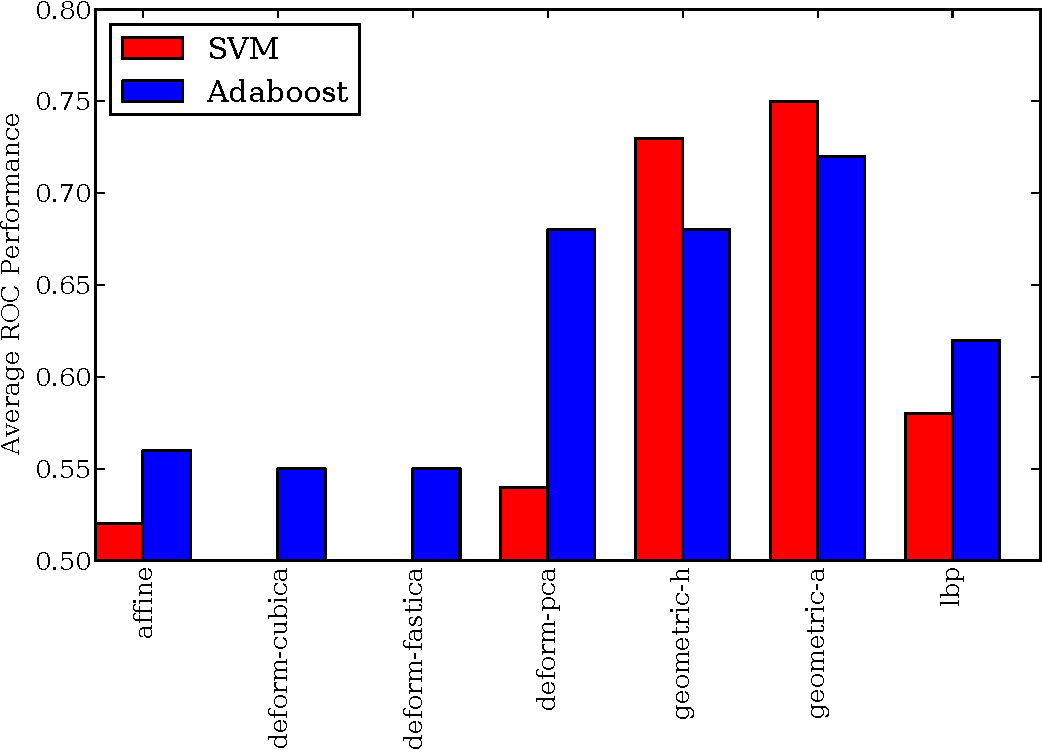
\includegraphics[width = 0.6 \columnwidth]{nvcclass/compare-multi-person.pdf}
\caption[Comparison of \textbf{multi-person} performance for different features.]{Comparison of \textbf{multi-person} performance for different features. Testing is at clip level, with the average score of all four \ac{NVC} categories. A performance of 0.5 is equivalent to classification by chance. SVM with geometric algorithmic features provides the best performance.}
\label{CompareGraphMultiPerson}
\end{figure}

\begin{figure}[tb]
\centering
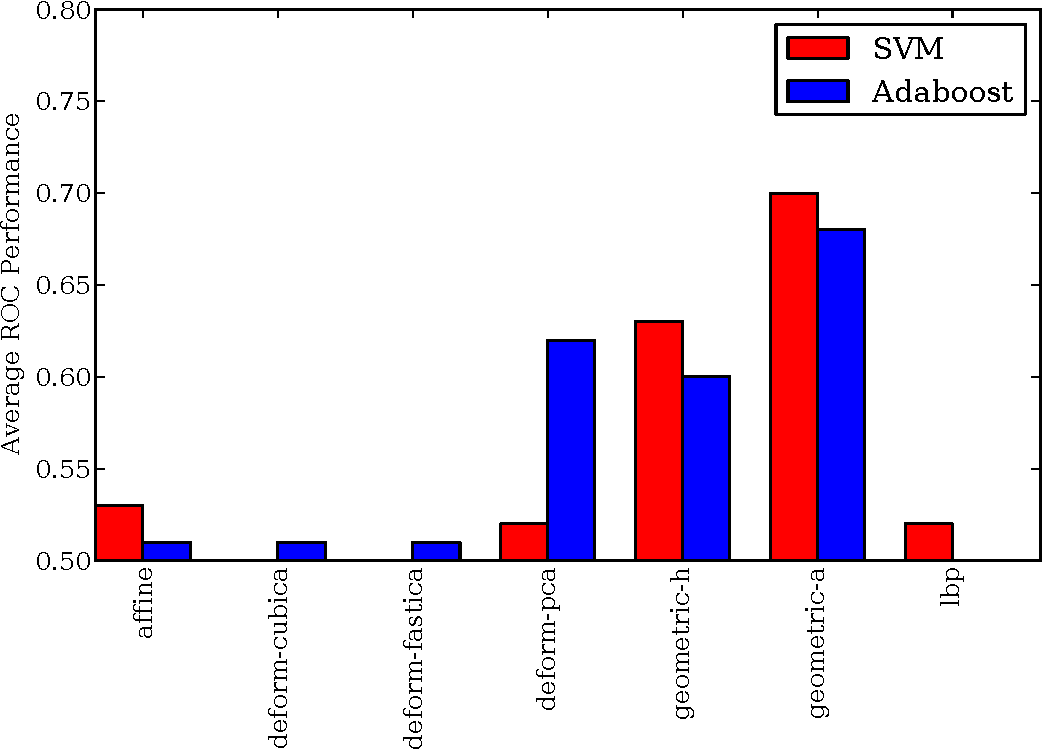
\includegraphics[width = 0.6 \columnwidth]{nvcclass/compare-person-indep.pdf}
\caption[Comparison of \textbf{person independent} performance for different features.]{Comparison of \textbf{person independent} performance for different features. Testing is at clip level, with the average score of all four \ac{NVC} categories. A performance of 0.5 is equivalent to classification by chance. SVM with geometric algorithmic features provides the best performance.}
\label{PersonIndependentCompareGraph}
\end{figure}

\thesiscomment{FIX graphs should be average area under ROC, y axis needs changing}

\thesisstatement{SVM is slightly better than Adaboost for NVC detection (forward channel)}

For the higher performing geometric features \textit{geometric-h} and \textit{geometric-a}, \ac{SVM} performance exceeds the performance for Adaboost. This may be due to information loss in the feature discretisation process, or \ac{SVM} was better suited to this task.

%The preceding paragraphs have discussed the combined performance for all four categories of \ac{NVC} signals (\textit{agree}, \textit{thinking}, etc.). They also have only dealt with clip level performance evaluation. However, 
The performance for each \ac{NVC} signal is of interest, because some \ac{NVC}s may be easier or harder to recognise automatically. 
%Also, clip level performance has been discussed, but comparing this with frame level performance should confirm the same general patterns. 
To limit the quantity of results to a manageable amount, only the top two approaches (SVM with \textit{geometric-a} and \textit{geometric-h}) are presented in the following discussion. Also, person independent testing is used exclusively, since this is a more challenging and general problem.

\begin{table}[tb]
\centering
\caption[\ac{AUC} Performance for algorithmic geometric features \textbf{\textit{geometric-a} using SVM} (person independent testing).]{Performance for algorithmic geometric features \textbf{\textit{geometric-a} using SVM} (person independent testing). Confidence intervals of two standard deviations are shown. Classification at the clip level provides better performance then frame level testing (but further tests are required to establish statistical significance). \textit{question} is the hardest NVC category to classify.}
\begin{tabular}{ c | c | c | c | c }
\hline
Testing & Agree & Question & Thinking & Understand\\
\hline
Clip level & 0.67$\pm$0.04 & 0.64$\pm$0.10 & 0.77$\pm$0.08 & 0.71$\pm$0.10\\ % XI
Frame level & 0.66$\pm$0.06 & 0.54$\pm$0.02 & 0.70$\pm$0.06 & 0.70$\pm$0.04\\ %X
\hline
\end{tabular}
\label{TableAlgorithmicFeatures}
\end{table}

\thesisstatement{Clip level classification is better than frame level regression}

\thesisstatement{Question and understand are harder to classify and regress than agree and thinking}

Table \ref{TableAlgorithmicFeatures} shows the \textit{geometric-a} SVM performance for the 4 \ac{NVC} categories for person independent testing. 
%The performances for different \ac{NVC} signals are shown in Table \ref{TableAlgorithmicFeatures} are also interesting. 
\textit{Thinking} appears to be the easiest \ac{NVC} signal to recognise, while \textit{question} is the hardest. 
%This is true in both clip level and frame level testing, which suggests that both performance metrics are somewhat similar. 
Low \textit{question} performance is probably due to the \ac{NVC} being primarily expressed by voice intonation \cite{Verderber2007} and sentence context, rather than any visual cue. Also, \textit{question} category contains fewer positive examples than the other \ac{NVC} signals in this study (Figure \ref{RatingScoresFigure}). Thinking has a characteristic visual appearance which is relatively easy to identify, as discussed in Section \ref{SectionVisualisingGaze}.
As previously observed, clip level classification reports a higher performance than frame level classification. %As discussed in Section \ref{SectionClassificationPerformance}, clip level testing produces a label based on a clip's overall content by decision level fusion. This is more effective than producing a set of possible prediction labels that each only consider a single frame.
However, it is difficult to establish the statistical significance of this result, due to the effect of personal differences increasing the variance of observed performance in the cross validation process. If this effect is ignored and \textit{thinking} \ac{NVC} is considered, clip level performance (0.77$\pm$0.04) exceeds the performance of frame level classification (0.70$\pm$0.03) with a significance of only $p=0.23$. Further experiments are required to establish if this result is statistically significant.

\begin{table}[tb]
\centering
\caption[\ac{AUC} Performance for heuristic geometric \textbf{\textit{geometric-h} features using SVM} classification (person independent testing).]{Performance for heuristic geometric \textbf{\textit{geometric-h} features using SVM} classification (person independent testing). Confidence intervals of two standard deviations are shown Clip level classification performance exceeds frame level performance. Although performance is generally lower than the use of algorithmic geometric features (Table \ref{TableAlgorithmicFeatures}), the \textit{agree} NVC performance is significantly better for heuristic geometric features.}
\begin{tabular}{ c | c | c | c | c }
\hline
Testing & Agree & Question & Thinking & Understand\\
\hline
Clip level & 0.73$\pm$0.08 & 0.54$\pm$0.16 & 0.58$\pm$0.00 & 0.68$\pm$0.16\\ % XI
Frame level & 0.59$\pm$0.04 & 0.51$\pm$0.04 & 0.52$\pm$0.04 & 0.56$\pm$0.04\\ %X
\hline
\end{tabular}
\label{TableHeuristicFeatures}
\end{table}

\thesisstatement{Different feature sets are better or worse on distinct types of NVC}

Moving from \textit{geometric-a} to \textit{geometric-h} features, which are shown in Table \ref{TableHeuristicFeatures}, the classification performance is significantly lower overall than in Table \ref{TableAlgorithmicFeatures}. However, the performance for \textit{thinking} in the case of \textit{geometric-h} exceeds features generated by \textit{geometric-a}. This shows that although \textit{geometric-a} is generally a good method for encoding different \ac{NVC} signals, it is not necessarily optimal for all types of \ac{NVC}. As above, statistical significance is low due to the effect of personal differences and further tests are required to establish significance.
%An extension of \textit{geometric-a} may result in a performance increase, by either including different types of features that make it similar to the heuristic features, or to apply feature selection. Chapter \ref{ChapterFeatureSelection} returns to the idea of feature selection for \textit{geometric-a}.

%This section has described testing based on classifying on individual frames and comparing these predictions with the annotation label. However, encoding of feature's variation over time can also be attempted. These \temporalFeatPlural are discussed in the next section.

\section{\temporalFeatPluralCap{ }using Quadratic Curve Fitting}
\label{SectionTemporalFeatures}

\diffblock{
\begin{figure}[tb]
\centering
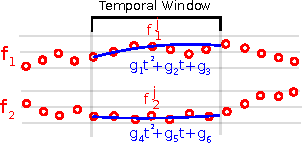
\includegraphics[width = 0.7 \columnwidth]{nvcclass/temporalFeatures.pdf}
\caption[Illustration of \temporalFeatPlural{ }for a simple two component frame feature with a single temporal window size.]{Illustration of \temporalFeatPlural{ }for a simple two component frame feature with a single temporal window size. A quadratic curve is fitted to samples in a sliding window. The parameters that describe the curve form part of the temporal vector. \thesiscomment{MathInFig}}
\label{FigureTemporalFeatures}
\end{figure}
}

%Although digital video data is usually recorded and accessed as a series of individual frames, considering frames in isolation is unlikely to be a good approach for \ac{NVC} recognition. 
Humans use the face shape and appearance variation in time for recognition of behaviour. 
Temporal variation of features should be investigated to attempt to achieve better automatic performance of emotion and \ac{NVC}.
This information is encoded by \temporalFeatPlural, which are defined here as the result of combining data from multiple sensor observations taken at a range of times. The temporal order of observations may be retained in the \featureGeneration process, or it may be discarded.
To create \temporalFeatPlural, each component of a clip feature (e.g. $\clipFeature_{geometric-h}$) is considered independently and in a sliding window (see Figure \ref{FigureTemporalFeatures}). A quadratic curve is fitted to the feature values in the sliding window $\temporalWindow$ of $\temporalWindowSize$ frames using least squares fitting $\temporalWindow \in \mathbb{R}^{\temporalWindowSize \times \numFeatures \times \numClipFrames}$. The parameters of the curve $\temporalWindowFeature$ are then used as the \temporalFeatSingle, which describes how a frame based feature varies over time in a temporal window $\temporalWindowFeature \in \mathbb{R}^{\numClipFrames \times 3 \numFeatures}$. This approach is related to Savitzky--Golay filtering \cite{Savitzky1964} and was previously used by Petridis and Pantic \cite{Petridis2008} to create \temporalFeatPlural{ }for laughter detection. 
%except that the polynomial coefficients are retained as features rather than used to reconstruct the signal. 
%The size of the frame feature matrix $\frameFeature$ for all the clips in a temporal window is $\numClipFrames$ frames by $\numFeatures$ features. 
%The size of \temporalFeatPlural for a single temporal window $\temporalWindowFeature$ is $\numClipFrames$ by $3 \numFeatures$ if quadratic polynomials are used. 
For the $i$th feature component $i \in \{1...\numFeatures\}$, at temporal window frame position $j$, $\timeOffset \in \{1...\temporalWindowSize\}, j \in \{1...\numClipFrames\}, \textbf{a} = \{\textbf{a}_{1}, \textbf{a}_{2}, \textbf{a}_{3}\}$:

\thesiscomment{TODO temporal window offset?}

\begin{gather}
\temporalWindow_{\timeOffset,i,j} = \clipFeature_{\timeOffset+j,i} \\
\polyFunc(\textbf{a},\timeOffset) = \textbf{a}_1 \timeOffset^2 + \textbf{a}_2 \timeOffset + \textbf{a}_3 \\
\{\temporalWindowFeature_{j,3i-2},\temporalWindowFeature_{j,3i-1},\temporalWindowFeature_{j,3i}\} = \argmin_{\textbf{a}} {\displaystyle\sum\limits_{\timeOffset=1}^{\temporalWindowSize} | \temporalWindow_{\timeOffset,i,j} - \polyFunc(\textbf{a},\timeOffset) |}
\end{gather}

Because the optimal size of the temporal window is unknown, multiple window sizes are used to form the \temporalFeatPlural. The number of temporal windows is denoted as $\numTemporalWindows$. The combined \temporalFeatSingle{ }$\temporalFeature$ is the concatenation of the various temporal windows, and the original frame feature $\frameFeature$ on frame $j$:

\begin{gather}
\temporalFeature_{j} = \{\frameFeature_1...\frameFeature_{\numFeatures},\temporalWindowFeature^1_{j,1}...\temporalWindowFeature^1_{j,3 \numFeatures},...,\temporalWindowFeature^\numTemporalWindows_{j,1}...\temporalWindowFeature^\numTemporalWindows_{j, 3 \numFeatures}\} \\
\temporalFeature \in \mathbb{R}^{\numClipFrames \times (3 \numTemporalWindows + 1) \numFeatures}
\end{gather}

The next section discusses their performance in \ac{NVC} classification.

\subsection{Results and Discussion}

The temporal window lengths used were 80ms, 160ms, 320ms and 640ms ($\numTemporalWindows = 4$). As before, five thresholds ($\numThresholds = 5$) were used for Adaboost classification. The SVM cost parameter $C$ of 1.0 was found to be effective.

\diffblock{
\begin{table}[tb]
\centering
\caption[Comparison of \ac{AUC} performance of \temporalFeatPlural{ }generated based on $\temporalFeature_{geometric-h}$.]{Comparison of \ac{AUC} performance of \temporalFeatPlural{ }generated based on $\temporalFeature_{geometric-h}$. SVM Classification was assessed by person independent testing. Confidence intervals of two standard deviations are shown}
\begin{tabular}{ c | c | c | c | c | c }
\hline
\temporalFeatPluralCap & Testing & Agree & Question & Think & Understand\\
\hline
No & Clip level & 0.73$\pm$0.08 & 0.54$\pm$0.16 & 0.58$\pm$0.00 & 0.68$\pm$0.16\\ % XI
\rowcolor[gray]{.95} Yes & Clip level & 0.74$\pm$0.06 & 0.57$\pm$0.10 & 0.60$\pm$0.04 & 0.69$\pm$0.12\\ % XI
No & Frame level & 0.59$\pm$0.04 & 0.51$\pm$0.04 & 0.52$\pm$0.04 & 0.56$\pm$0.04\\ %X
Yes & Frame level & 0.60$\pm$0.04 & 0.51$\pm$0.04 & 0.55$\pm$0.04 & 0.58$\pm$0.04\\ % X
\hline
\end{tabular}
\label{TableHeuristicFeaturesTemporal}
\end{table}
}

\thesisstatement{Polynomial \temporalFeatPlural{ }do not significantly improve NVC classification}

The performance of \temporalFeatPlural{ }is shown in Table \ref{TableHeuristicFeaturesTemporal}. Heuristic features $\temporalFeature_{geometric-h}$ were used instead of $\temporalFeature_{geometric-a}$ features because its feature matrix is extremely large and exceeds available computer memory resources. The usage of \temporalFeatPlural{ }only results in a slight or negligible improvement in performance in both clip and frame level testing, however further tests are required to establish statistical significance. 
%This implies that the extra information encoded by this form of \temporalFeatPlural do not provide a large improvement to \ac{NVC} classification. 
The performance improvement may be due to input smoothing rather than the linear or quadratic terms in the polynomial being useful. This possibility is supported by feature weights assigned in an Adaboost strong classifier; quadratic and linear terms are generally not selected. In the work by Petridis and Pantic \cite{Petridis2008}, tests showed performance was not significantly affected by varying the temporal window size (Table 2 in their paper). However, humans require temporal information to identify complex emotion, so it is unlikely that temporal information has no role in \ac{NVC}. Other approaches to \temporalFeatPlural{ }and classification are investigated in Sections \ref{SectionHmm} and \ref{SectionClipFeatureExtraction}.

%\section{Feature Selection for NVC Classification}
%\label{SectionClassificationFeatureSelection}

%\thesisstatement{Certain features were consistently selected by Adaboost}

%DISCUSS: What features are selected by Adaboost?


%The next section examines human behaviour during \textit{thinking} and sees how this is encoded in feature space.

\section{Visualising Gaze Features during Thinking}
\label{SectionVisualisingGaze}

\thesisstatement{Apart from the mean and variance of the trajectory in feature space, there is little consistency between different thinking examples.}

\begin{figure}[tb]
\centering
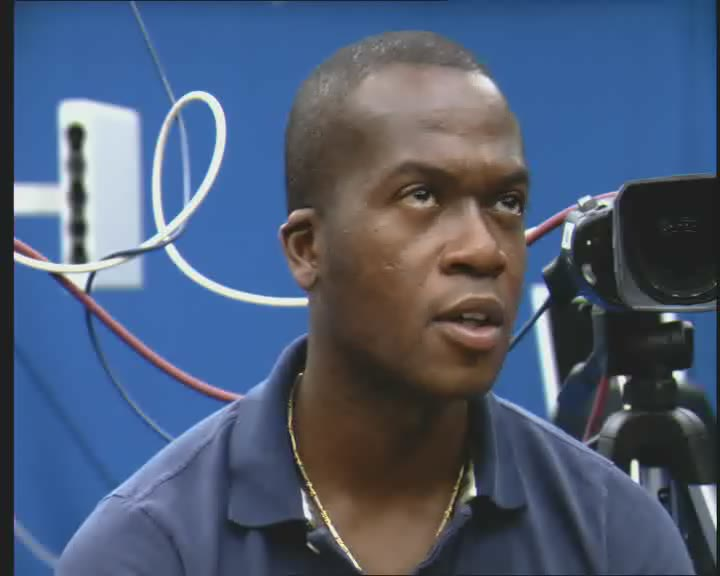
\includegraphics[width = 0.49 \columnwidth]{nvcclass/pos_thinking_clip_0ikEnNwEiH.jpg}
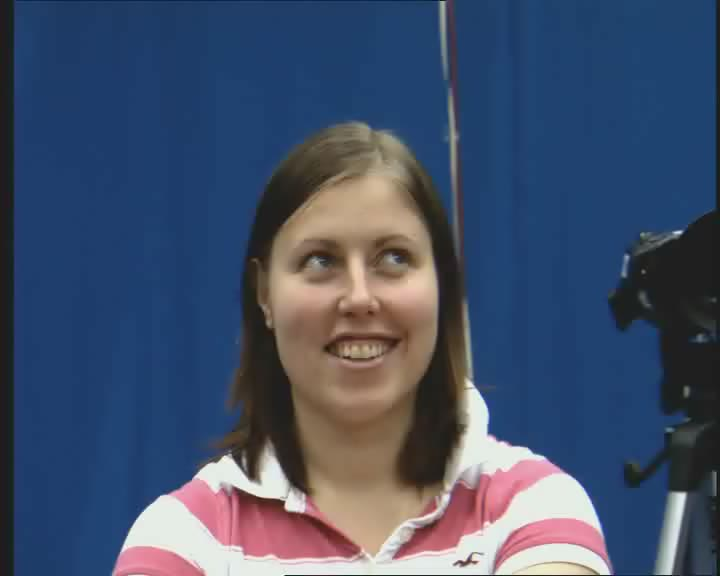
\includegraphics[width = 0.49 \columnwidth]{nvcclass/pos_thinking_clip_1HrHJGReu2.jpg}

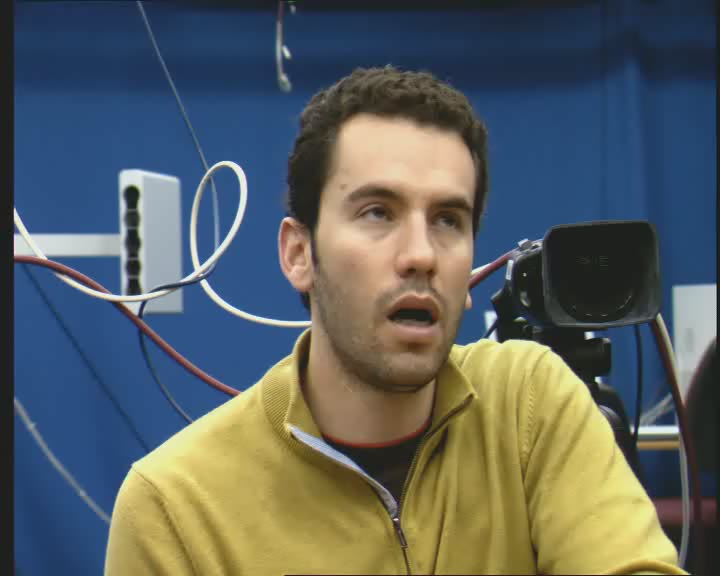
\includegraphics[width = 0.49 \columnwidth]{nvcclass/pos_thinking_clip_G3N4eNTLUH.jpg}
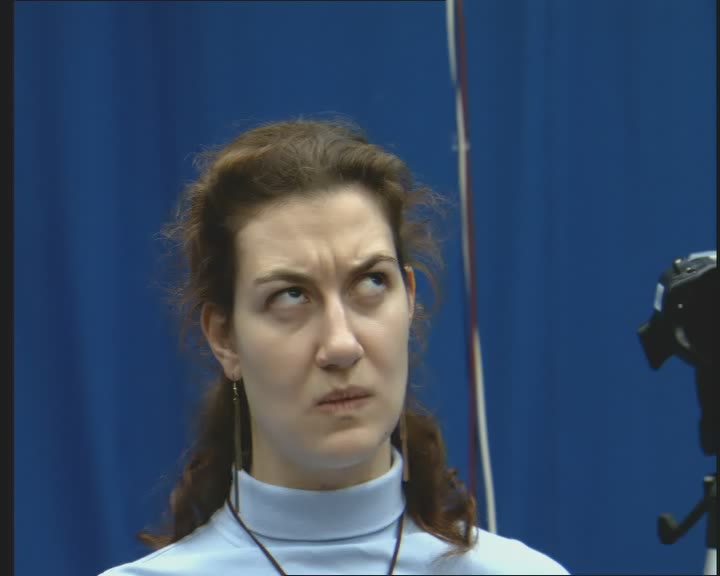
\includegraphics[width = 0.49 \columnwidth]{nvcclass/pos_thinking_clip_t8jTJw1Zrs.jpg}
\caption[Frames from the top 4 annotator rated examples of positive \textit{thinking}.]{Frames from the top 4 annotator rated examples of positive \textit{thinking}. Averted gaze is strongly expressed in positive examples of \textit{thinking}. The specific frames from the clip were manually selected.}
\label{FigurePosThinkingGbr}
\end{figure}

\begin{figure}[tb]
\centering
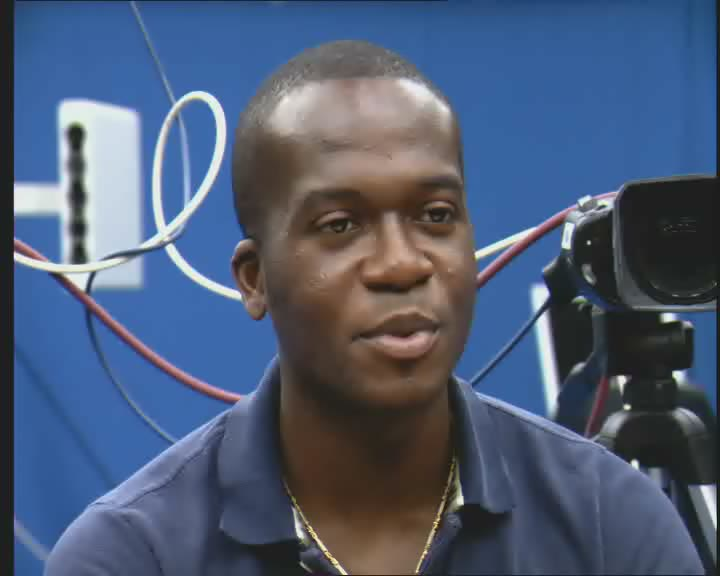
\includegraphics[width = 0.49 \columnwidth]{nvcclass/neg_thinking_clip_9B4pDQJIUC.jpg}
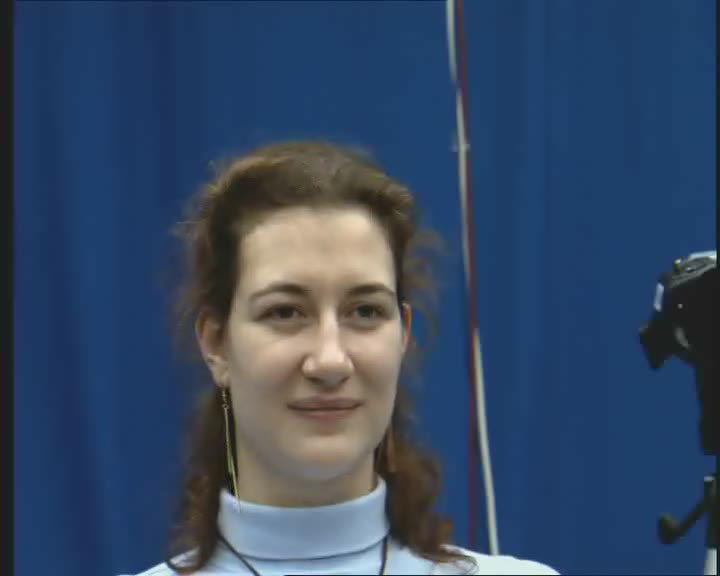
\includegraphics[width = 0.49 \columnwidth]{nvcclass/neg_thinking_clip_BShb9DBvU0.jpg}

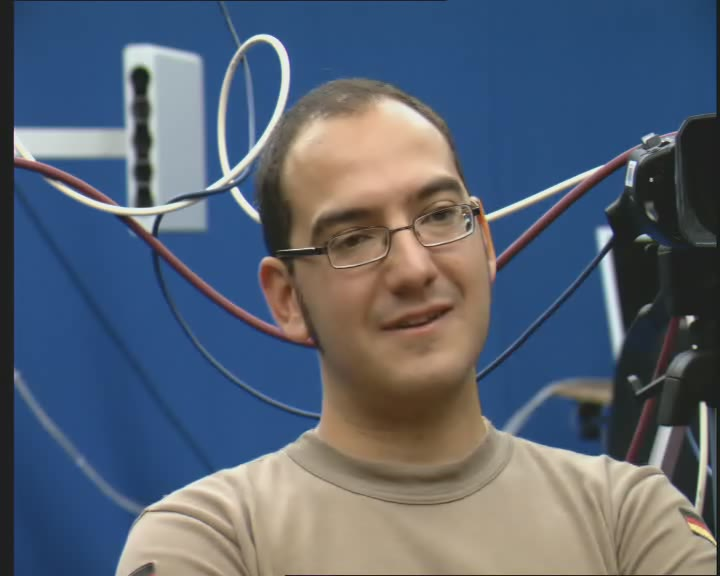
\includegraphics[width = 0.49 \columnwidth]{nvcclass/neg_thinking_clip_CTIOfHcxSt.jpg}
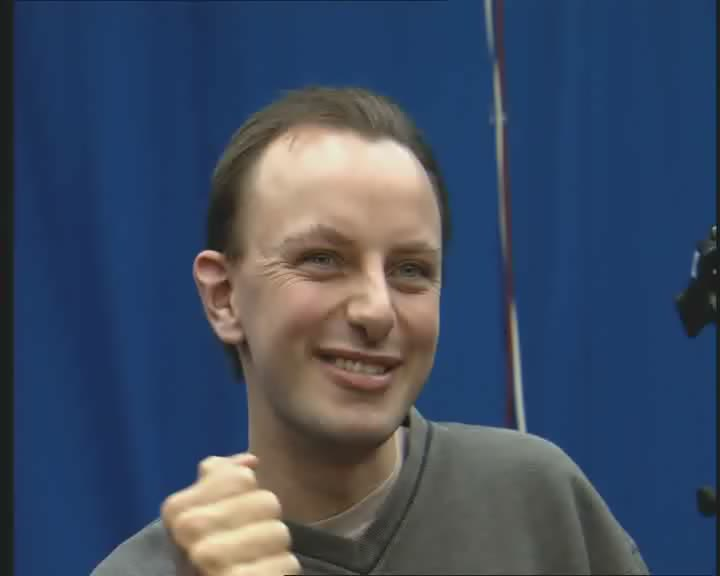
\includegraphics[width = 0.49 \columnwidth]{nvcclass/neg_thinking_clip_DGUb6od8BB.jpg}
\caption[Frames from the top 4 annotator rated examples of negative \textit{thinking}, i.e. \textit{thinking} is not present.]{Frames from the top 4 annotator rated examples of negative \textit{thinking}, i.e. \textit{thinking} is not present. Eye contact is maintained in negative examples of \textit{thinking}. The specific frames from the clip were manually selected.}
\label{FigureNegThinkingGbr}
\end{figure}

%The previous section described several approaches to encode facial feature deformations and appearance. 
This section will consider a simplified problem that is intended to provide insight into how \ac{NVC} signals are manifested in feature space. This can inform the decision on how to approach the problem. The \ac{NVC} for \textit{thinking} is used, because clear positive and negative examples of this signal have a distinctive gaze pattern. This has previously been observed in various studies, such as McCarthy \etal \cite{McCarthy2006}, which found that eye contact was broken when a person is thinking about how to answer a question (see Figures \ref{FigurePosThinkingGbr} and \ref{FigureNegThinkingGbr}). 
%The effect is visible examples that were rated as strongly positive \textit{thinking} (Figure \ref{FigurePosThinkingGbr}) which contrasts starkly with strongly negative \textit{thinking} (Figure \ref{FigureNegThinkingGbr}). Examples that were rated as negative \textit{thinking} maintained eye contact through out the video clip. This consistent behaviour pattern can be easily encoded with distance features based on eye tracking. 

Two features from heuristic geometric features, introduced in Section \ref{SectionGenerateHeuristic}, are used to encode eye movements. Using the full \textit{geometric-h} feature vector would be difficult to visualise as a 2{D} plot, so the 2 features that are relevant are manually selected. The 9th and 12th feature of \textit{geometric-h} corresponds to ``Mean eye horizontal'' and ``Mean eye vertical'' positions respectively (see Table \ref{GeometryFeaturesTable}), which will be referred to as the ``gaze subset''. These simple features can be used to visualised positive and negative samples.

\begin{figure}[tb]
\centering
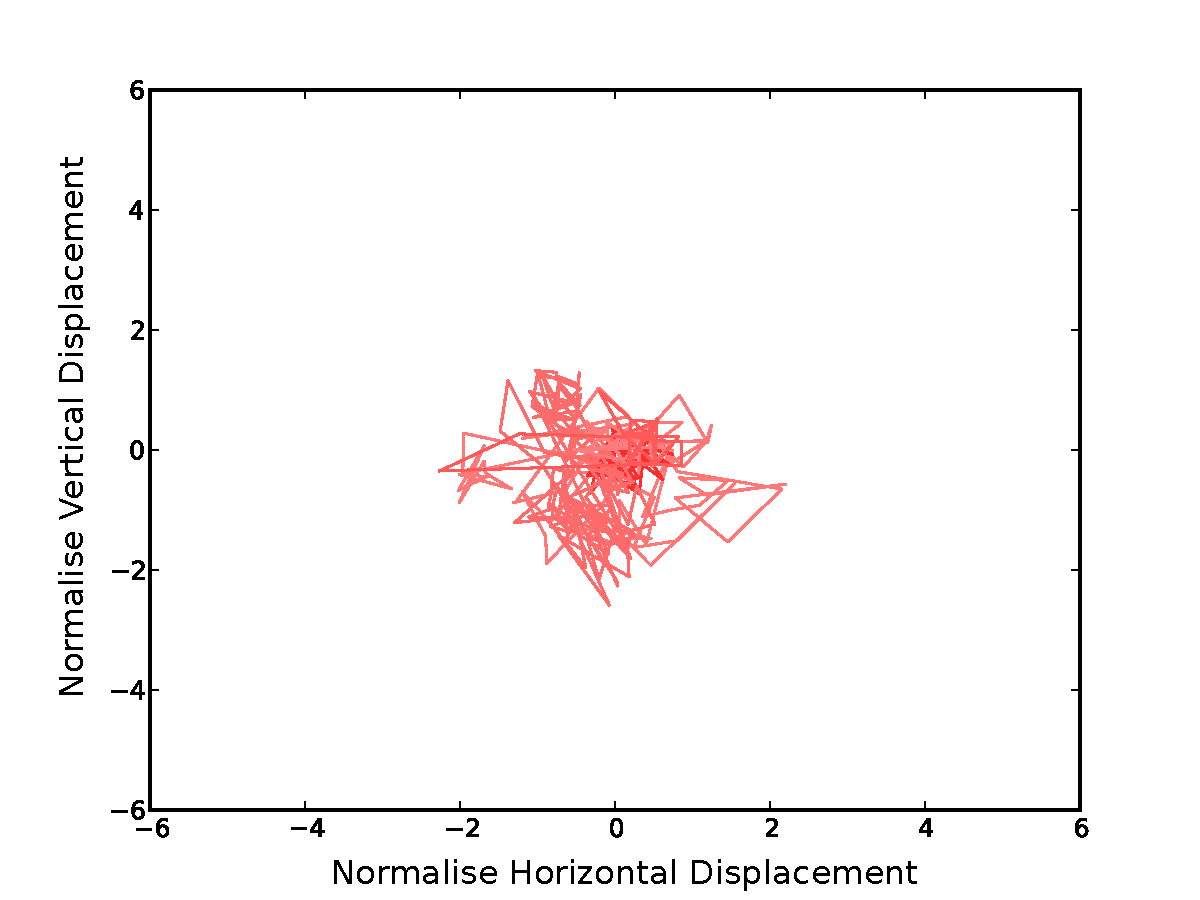
\includegraphics[width = 0.49 \columnwidth]{nvcclass/traj0.pdf}
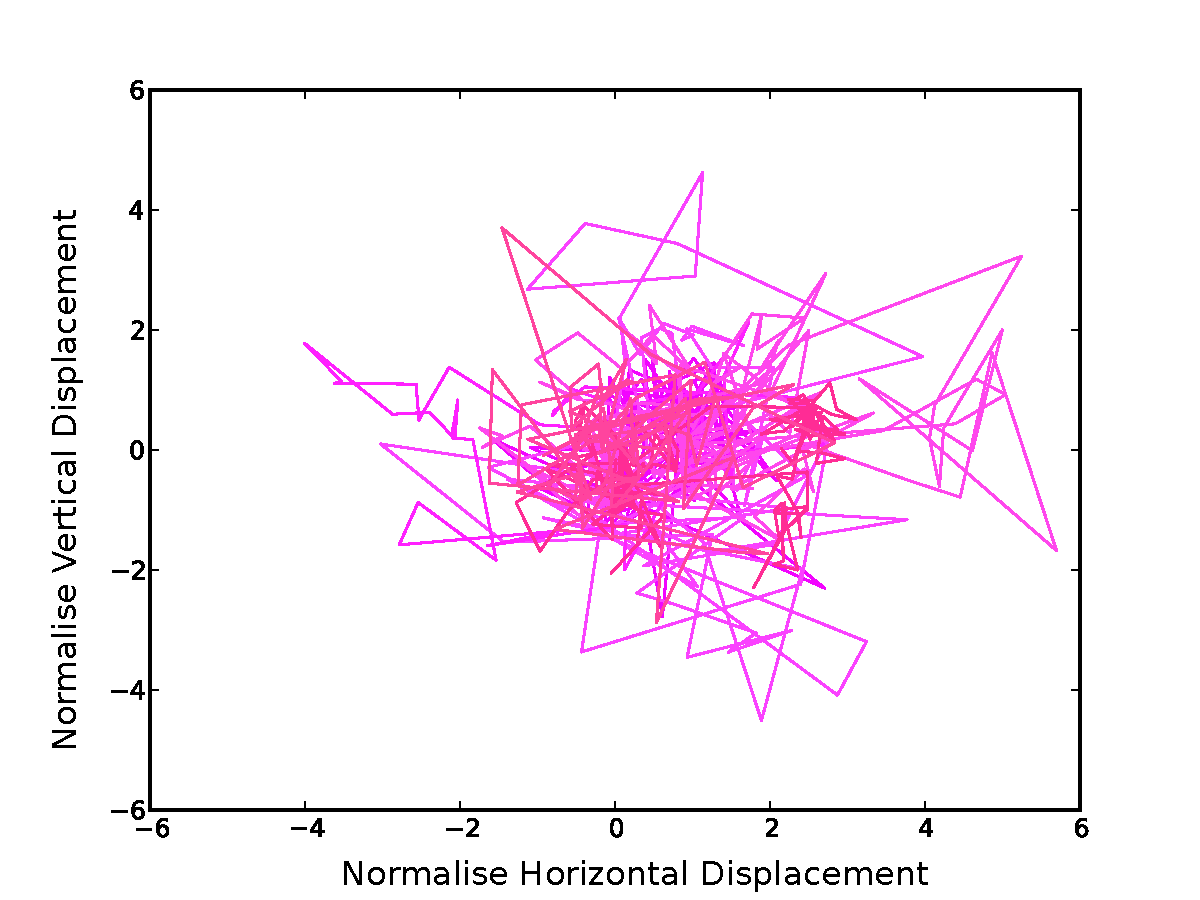
\includegraphics[width = 0.49 \columnwidth]{nvcclass/traj99.pdf}
\caption[Eye trajectories in the top 1\% positive and top 1\% negative examples of \textit{thinking}.]{Eye trajectories in the top 1\% positive and top 1\% negative examples of \textit{thinking}. The left plot shows the negative examples. The right plot shows the positive examples. The trajectory shape in the plot correspond to observed eye motion i.e. the top of the plot corresponds to looking upwards. Differences in line shading correspond to different video samples.}
\label{FigureThinkingTrajectoryPosNeg}
\end{figure}

Each annotated example is a video clip containing multiple frames. The gaze subset of \textit{geometric-h} encode each frame as a 2 component vector. This trajectory is shown in Figure \ref{FigureThinkingTrajectoryPosNeg} as a 2D plot. As can be seen, gaze in negative examples is relatively steady and is generally near the origin, which corresponds to frontal gaze. Any motion away from the origin is due to eye motion or tracker noise. Gaze in positive examples of thinking contain significantly more variation and excursions from the origin to the upper right in the plot. This corresponds to the characteristic thinking behaviour seen in Figure \ref{FigurePosThinkingGbr}. This makes positive and negative examples quite distinct in feature space. These patterns in eye movement are likely to be used for automatic \textit{thinking} recognition (this is verified in Section \ref{SectionVisualiseFeatureSelection}).

\begin{figure}[tb]
\centering
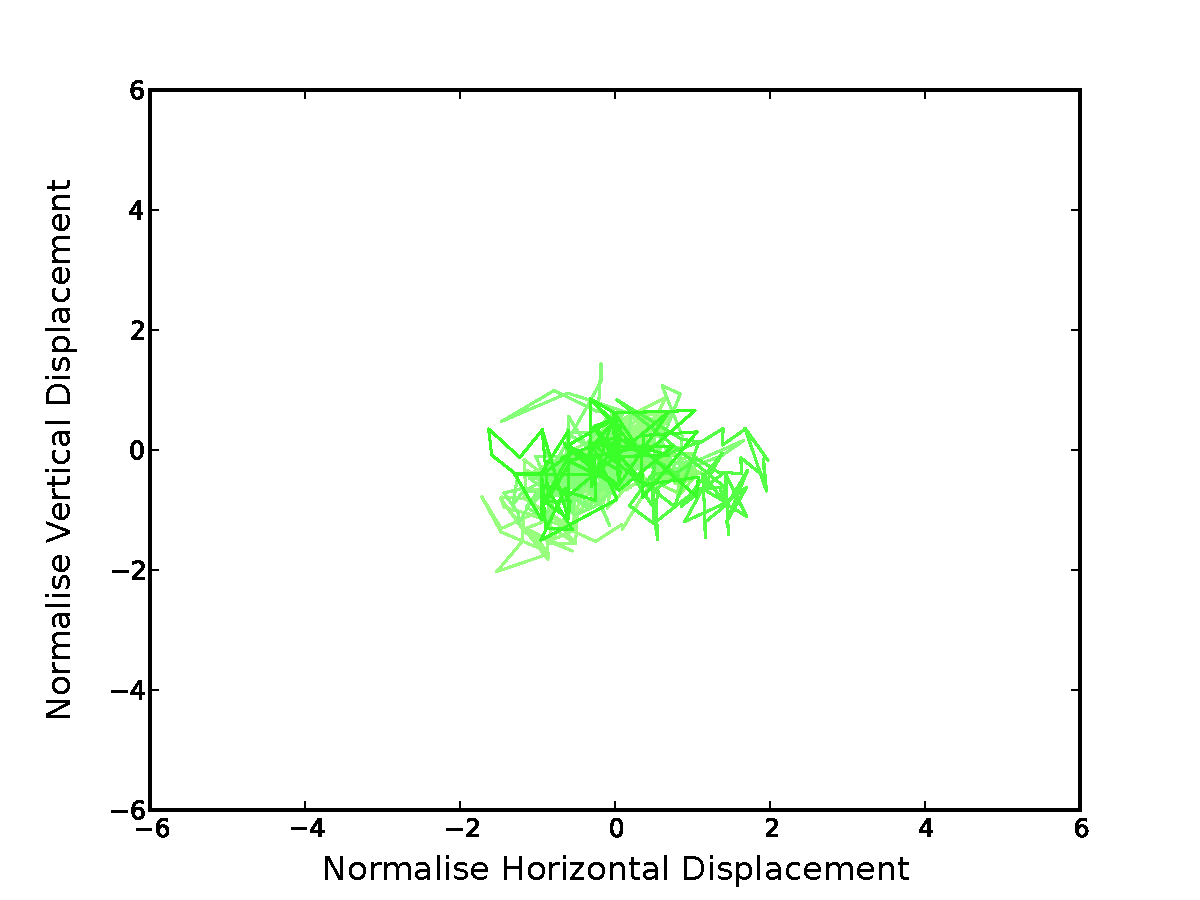
\includegraphics[width = 0.49 \columnwidth]{nvcclass/traj50.pdf}
\caption[Eye trajectories in the middle 1\% examples of \textit{thinking}.]{Eye trajectories in the middle 1\% examples of \textit{thinking}. The trajectory shape in the plot correspond to observed eye motion i.e. the top of the plot corresponds to looking upwards. Differences in line shading correspond to different video samples.}
\label{FigureThinkingTrajectoryIntermediate}
\end{figure}

While positive and negative examples are easy to distinguish, intermediate strength examples of \textit{thinking} may prove challenging, if the gaze behaviour is not distinct in gaze feature space. The trajectories of the middle 1\% intensity of \textit{thinking} is shown in Figure \ref{FigureThinkingTrajectoryIntermediate}. As can be seen, the trajectories are not significantly different from negative samples shown in the left plot of Figure \ref{FigureThinkingTrajectoryPosNeg}. This lack of difference may make differentiating between intermediate and negative examples problematic. %Currently, only a greatly simplified example limited to 2 features is considered and this chapter is only concerned with clear examples of \ac{NVC}. Later chapters address intermediate intensity \ac{NVC}. However, use of additional features may provide additional information that enables reliable discrimination of various intensities of \ac{NVC}.

\begin{figure}[tb]
\centering
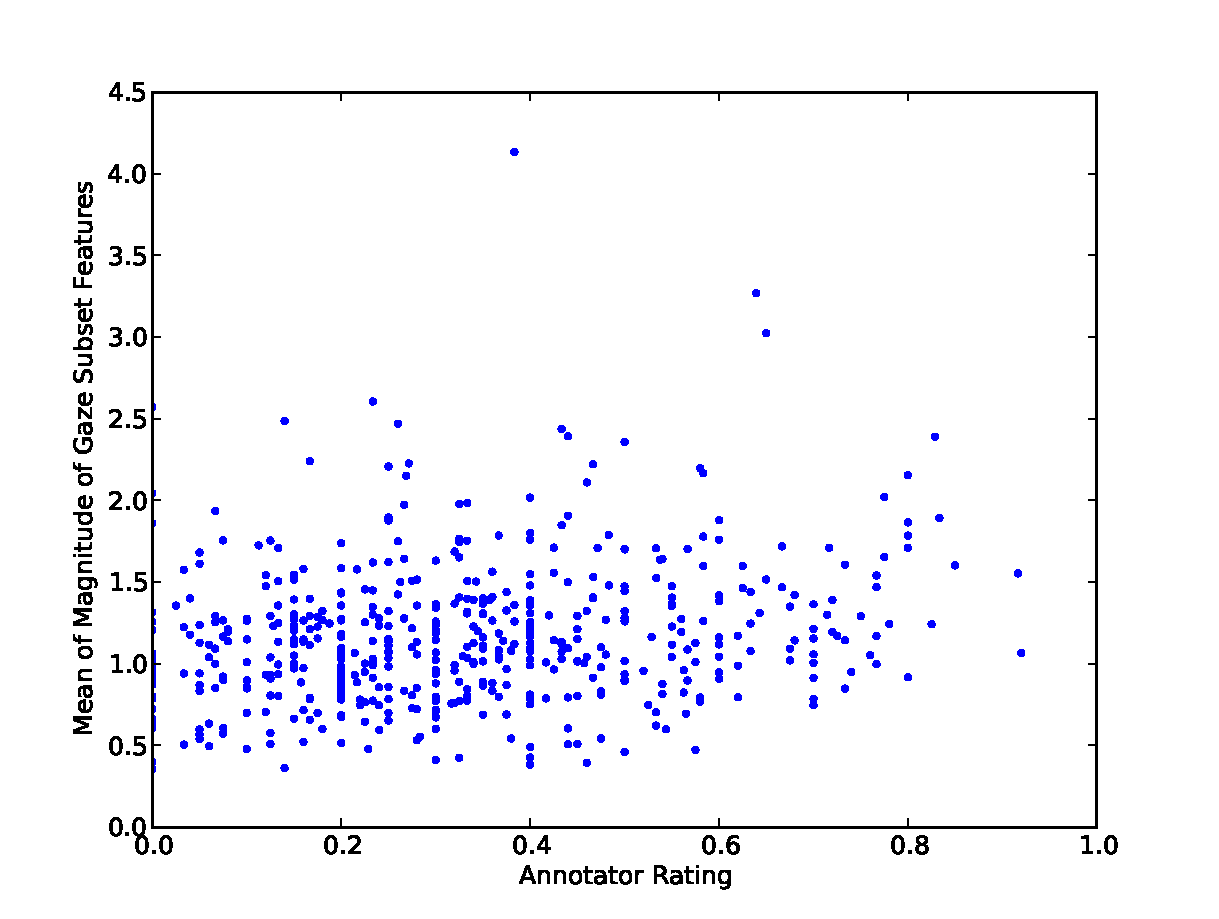
\includegraphics[width = 0.7 \columnwidth]{nvcclass/ThinkingGazeMean.pdf}
\caption[The mean magnitude of the gaze features for each clip $\clipFeatureDigestVal$, plotted against the annotator rating of \textit{thinking}.]{The mean magnitude of the gaze features for each clip $\clipFeatureDigestVal$, plotted against the annotator rating of \textit{thinking}. There is a weak linear trend between increasing feature magnitude and the intensity of \textit{thinking}.}
\label{FigureThinkingMeanScatter}
\end{figure}

%\begin{figure}[tb]
%\centering
%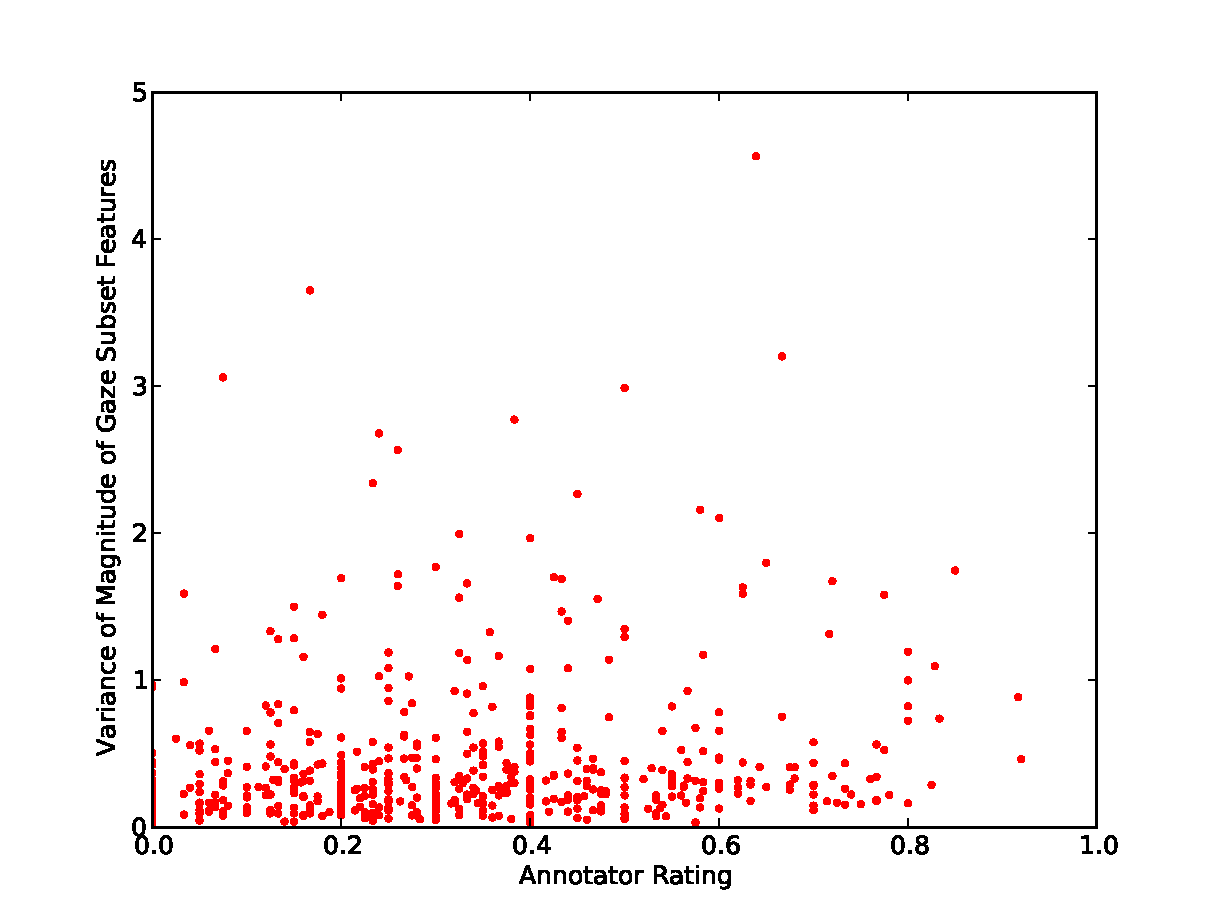
\includegraphics[width = 0.7 \columnwidth]{nvcclass/ThinkingGazeVar.pdf}
%\caption{}
%\label{FigureThinkingVarScatter}
%\end{figure}

The feature can be further simplified by computing the average magnitude of eye deviation from frontal gaze. This also enables representation of a clip by a single number $\clipFeatureDigestVal \in \mathbb{R}$:

\begin{gather}
\clipFeatureDigestVal = %\overline{\sqrt{(\clipFeature_{geometric-h}}_{9}^{\frameNum})^2 + (\clipFeature_{geometric-h}_{12}^{\frameNum})^2}}
\frac{\displaystyle\sum\limits_{j=1}^{\numClipFrames} \sqrt{{\clipFeature_{geometric-h,j,9}}^2 + {\clipFeature_{geometric-h,j,12}}^2}}
{\numClipFrames}
\end{gather}

Figures \ref{FigureThinkingTrajectoryPosNeg} and \ref{FigureThinkingTrajectoryIntermediate} only show the trajectories for a small subset of samples. With the mean clip feature $\clipFeatureDigestVal$, the feature can be plotted against the annotator rating for all samples in the corpus (Figure \ref{FigureThinkingMeanScatter}). As can be seen, there is only a weak linear association between this gaze subset feature and the annotators score. The correlation of the feature with the annotation is $0.21$. This illustrates the difficulty in \ac{NVC} recognition: there is little consistency in human behaviour and while particular facial actions may have statistical connections with \ac{NVC}, they are not definitive. 
%By examining the clear examples, which are the left-most and right-most 25 samples in the plot, it can be seen they are generally separable by a threshold of about $\clipFeature_{mean}=1.0$. The rest of the chapter continues with describing and evaluating an automatic \ac{NVC} classification system.
%This section has shown that for possibly the easiest \ac{NVC} signal, \textit{thinking}, and with manually selected gaze features it is possible to distinguish clear examples but, it is difficult to separate intermediate examples of \ac{NVC}. The other \ac{NVC} categories are considered, this problem is likely to be magnified because it is difficult to manually select or design an appropriate feature. For example, it is not immediately obvious, even for a human, how to identify what visual cues are associated with \textit{question}. Also, if intermediate strength clips are considered, it is difficult to distinguish intermediate intensity examples from strong and weak intensity \ac{NVC}, even in a simplified case. This is in stark contrast to many classic problems in computer vision, where at least some distinguishing characteristics of different classes are usually obvious and candidate features may be manually select to create a reasonably effective system. 
Section \ref{SectionDigestVector}  returns to the concept of summarising an entire clip by a single vector. However, it is important to consider this work in the context of the extreme difficulty of the problem.

\section{Discussion of Akak{\i}n and Sankur, 2011}
\label{SectionHmm}

\thesiscomment{Move self situation to front?}

An early version of the work in this chapter was published in 2009 \cite{SheermanChase2009}. A later paper by Akak{\i}n and Sankur \cite{Akakin2011} used the TwoTalk corpus, as well as the BUHMAP database \cite{Aran2007} to compare approaches to automatic recognition. 
%Their findings support some of the assumptions made in this chapter. They also provide additional insight in their conclusions that compliment the previous sections in this chapter. 
Because of the high relevance of their work to this thesis, this section outlines their approach, and discusses their conclusions in light of more recent work.

Their tracking is based on a detection-track-regularise framework with multiple tracking models to account for head pose changes. They used 1208 training frames, which has a higher manual training requirement than \ac{LP} tracking. Their approach is likely to have better recovery after occlusion and less manual intervention when in operation. The tracking is then used to  generate features: landmark coordinate features, heuristic geometric features, and texture features generated from localised patches. These broad types of features are the same as used in Section \ref{SectionFeatureGeneration}.%, although Akak{\i}n and Sankur use different texture descriptors and slightly different heuristic features.

%In  contrast to Section \ref{SectionNvcClassificationResults}, they attempt to model the temporal variations based on supervised learning techniques. 
They use two broad types of machine learning: feature-sequence classifiers (\ac{HMM}, \ac{HCRF}) and feature subspace learning (\ac{ICA} or \ac{NMF}, classified by \ac{MNN}). A key difference between these methods is feature-sequence classifiers consider the frame order as significant, while feature subspace learning does not. The use of \ac{MNN} is interesting because it allows direct comparison of an entire trajectory with another trajectory. 
%However nearest neighbour methods have a potential difficulty ignoring irrelevant features, which is the likely reason the experimenter chose to manually tune the number of features used in classification. 
The authors provide a justification for using feature-sequence methods by claiming that ``even though head and facial gestures may differ in total duration, each follows a fixed pattern of temporal order''. While specific gestures generally have a set pattern, it is possible that a particular \ac{NVC} signal may be expressed by more than one type of gesture.
%Although most head gestures are temporal in nature, such as nodding for agreement, human behaviour is more complex then following a set pattern to express an emotion or \ac{NVC} signal. The ordering of gaze changes, head pose movements and facial deformations is highly variable between humans and even for a single human (see discussion of the variability of gaze behaviour in Section \ref{SectionVisualisingGaze}). So, even if posed human behaviour ``follows a fixed pattern'', the same is not necessarily true for spontaneous human behaviour.

\begin{table}[tb]
\centering
\caption[\ac{AUC} performance on the TwoTalk corpus, expressed as percentages.]{\ac{AUC} performance on the TwoTalk corpus, expressed as percentages. The first four rows are from Table 11 in Akak{\i}n and Sankur, 2011 \cite{Akakin2011} and are quoted verbatim. Testing is multi-person. Results from \textit{geometric-a} with an SVM classifier have been appended for comparison (multi-person, clip level testing) (see Table \ref{TableCompareFeaturesAndClassifiers} and \ref{SvmClipMultipersonTable}).}
\begin{tabular}{ c || c | c | c | c | c }
Method & Agree & Question & Thinking & Understand & Average \\
\hline
MNN with ICA (P) & 84.6 & 67.6 & 83.5 & 74.3 & 77.5 \\
MNN with NMF (P) & 75.8 & 60   & 76.1 & 77.8 & 72.4 \\
HCRF (17,G)      & 78.7 & 75   & 73.5 & 82.5 & 77.4 \\
Classifier Fusion & 85.9 & 78.2 & 83.8 & 83.6 & 82.9 \\
\hline
Fused Features, Adaboost & 70 & 73 & 81 & 80 & 76 \\
\textit{geometric-a}, SVM & 70 & 70 & 83 & 75 & 75 \\
\end{tabular}
\label{TableCompareToAkakin}
\end{table}

The results from Akak{\i}n and Sankur are reproduced in Table \ref{TableCompareToAkakin}. All the results presented in the comparison were based on evaluation with the TwoTalk corpus.
%The first four results correspond to the performance of their system on the TwoTalk corpus. 
This table refers to a hybrid approach which is an early version of the approach described in this chapter (see \cite{SheermanChase2009} for details). This hybrid approach is a concatenation of the features $\frameFeature_{pca}$, $\frameFeature_{geometric-h}$, $\frameFeature_{lma}$ and $\frameFeature_{affine}$ with polynomial temporal fitting applied (see Section \ref{SectionTemporalFeatures}) with Adaboost. The final row in the table corresponds to the method described in this chapter ($\frameFeature_{geometric-a}$ and an \ac{SVM} classifier). As can be seen, the non-hybrid approaches methods have similar levels of performance. The use of a single type of sequential classifiers (MNN or HCRF) only results in 2 to 3\% improvement over the \textit{geometric-a} with the \ac{SVM} approach. 
%This implies that these sequential classifiers (\ac{HMM} and \ac{HCRF}) do not perform significantly better than non-sequential approaches, despite these methods being popular in emotion recognition. 

Comparing the non-fused approaches, the best approach for each \ac{NVC} category are MNN with ICA for \textit{agree} and \textit{thinking}, and HCRF for \textit{question} and \textit{understand}. MNN is poor for \textit{question} \ac{NVC} and HCRF is relatively poor for \textit{thinking}. The method proposed in this chapter (\textit{geometric-a}, SVM, see Table \ref{TableCompareFeaturesAndClassifiers}) has an overall performance that is comparable with these non-fused approaches but is worse for \textit{agree} than the temporal modelling approaches. Further tests would be required to establish statistical significance but it is likely that there is little difference in performance between these methods overall. Differences in specific \ac{NVC} category performance may be due to:
\begin{itemize}
 \item Each method uses a different representation of the face shape, with each being effective for recognizing a particular subset of \ac{NVC} signals.
 \item Temporal modelling may be beneficial for recognizing motion, such as nodding in \textit{agree} which may account for its advantage in performance.
 \item A \featureGeneration approach may be advantageous if a particular \ac{NVC} cannot be characterised by a consistent series of face shapes.
\end{itemize}

The absence of performance improvement using temporal modelling is similar Petridis \etal \cite{Petridis2009}, who concluded that while the field has moved towards ``advanced data fusion methods relying on dynamic classifiers'' for human behaviour recognition, the results from their experiments show that the supposed advantage of dynamic classifiers over static classifiers is ``not straightforward and depends on the feature representation [...] and the task at hand''. In the context of their study, ``HMMs does not seem to be beneficial, since it achieves the same performance as a static model''.
Also in the FERA2011 Facial Expression Recognition and Analysis Challenge \cite{Valstar2011}, Yang and Bhanu's approach was the most effective in both the person independent and overall evaluation and did not temporally model emotions but rather combined a video frames into an emotional avatar frame \cite{Yang2011}.
%who concluded the \featureGeneration was more significant than the distinction between static vs. dynamic classification methods. 
%This may be partly due to temporal variations being modelled at the \featureGeneration stage.
%Their classifier fusion approach is currently the best performer for \ac{NVC} classification. A similar pattern is observed when methods presented in this chapter are combined by feature fusion. However, 
Hybrid approaches that combine dynamic and static classification were not used in this thesis but often have higher performance than non-hybrid methods. 
%Given that \ac{NVC} recognition is a relatively new area with a significant number of unsolved issues, this possible confusion was avoided. However, for a practical system which requires maximum performance, it is probable that a hybrid system would be more effective than just using a single \featureGeneration method.
Interestingly, based on their BUHMAP based tests, Akak{\i}n and Sankur conclude that geometric features are superior to texture based features in both sequential and subspace classifiers. This finding concurs with the results presented in this chapter. 
%This is interesting, considering that many other papers which investigate emotion recognition often use facial appearance features only.
%The Akak{\i}n and Sankur results on the TwoTalk corpus used the same testing methodology as our earlier paper, in that they are multi-person cross validation tests. This raises the question as to their transferability to person-independent testing. As can be seen in Table \ref{TableCompareFeaturesAndClassifiers}, several promising approaches are not effective in person-independent tests. The Akak{\i}n and Sankur methods tested on BUHMAP by the person-independent protocol and seem to generalise well. However, the BUHMAP and TwoTalk corpuses are quite different: one being pose and the other is spontaneous. In this work, it was found that neither heuristic geometric features, nor using tracking data directly, was particularly effective at person-independent tests on TwoTalk, which forms the basis for Akak{\i}n and Sankur's higher performing approaches. This difficulty was the primary reason why \textit{geometric-a} features were created. However, their heuristic features encode different information than the \textit{geometric-h} features. It would be interesting to see how their approaches fare in person-independent tests on the TwoTalk corpus.
%The work of Akak{\i}n and Sankur are broadly in agreement with the findings of this chapter. 
%Conclusions will now be drawn, based on the work presented in this chapter.
Binary classification of clear examples of \ac{NVC} is re-examined in Section \ref{SectionDigestVectorOnClassification}. 

\section{Conclusion}

This chapter is a study of automatic classification for common, clear \ac{NVC} signals in informal conversations. Various \featureGeneration approaches are compared, as well as two classifiers. The best performance is achieved by a shape based geometric feature that exhaustively computes distances between pairs of trackers. 
%This provides good generalisation to person independent classification of \ac{NVC}. 
However the method does not encode temporal information in the classifier model. Temporal encoding of feature variations using polynomial curve fitting was not found to increase performance significantly. Also, person specific normalisation of features was only applied to the algorithmic geometric features, and not to the other \featureGeneration methods. Person specific normalisation should greatly benefit appearance features such as \ac{LBP} because of the differences in facial appearance across different people can be removed and generalisation can be improved. Later chapters improve on the work here in that they have person specific normalisation applied uniformly to all \featureGeneration methods.

In this study, shape is found to be more effective than appearance features, which agrees with similar findings in other papers \cite{Akakin2011} \cite{Lucey2009}, although some studies found appearance based features at least as significant \cite{Luettin1996} \cite{Valstar2011slides}. 
%This is partly down to differences in the task and also by each approach uses different shape or appearance features. This is interesting because only a few papers compare shape and appearance based features. 
%Almost every comparison that includes multiple features that are fused has found that this significantly improves performance. Also, the use of fusion of different classifiers, encoding of non-facial visual information and the addition of other modes may significantly improve performance. 

%This system operates on naturalistic data that was recorded with the minimum of constraints, however it may be better to record human interaction outside the laboratory setting to avoid reactivity. 
The differences in cultural background in both the emotional encoders (the people who expressed the \ac{NVC}) and the annotators (the people who perceived the \ac{NVC}) is not considered. Cultural differences in \ac{NVC} perception are revisited in Chapter \ref{ChapterAnnotation}, in which \culturallySpecific annotation data is collected. 
%\ac{NVC} has been considered as a simplified two class problem on clear examples. This constraint is removed and the problem is re-examined as a regression problem in Chapter \ref{ChapterNvcRegression}. 
The next chapter attempts to create an \ac{NVC} recognition system based on communication backchannel, which loosely speaking is a ``\ac{NVC} listener's'' response to a communication event.
